% Options for packages loaded elsewhere
\PassOptionsToPackage{unicode}{hyperref}
\PassOptionsToPackage{hyphens}{url}
\PassOptionsToPackage{dvipsnames,svgnames,x11names}{xcolor}
%
\documentclass[
  11pt,
  ignorenonframetext,
  dvipsnames,UTF8]{beamer}
\usepackage{pgfpages}
\setbeamertemplate{caption}[numbered]
\setbeamertemplate{caption label separator}{: }
\setbeamercolor{caption name}{fg=normal text.fg}
\beamertemplatenavigationsymbolsempty
% Prevent slide breaks in the middle of a paragraph
\widowpenalties 1 10000
\raggedbottom
\setbeamertemplate{part page}{
  \centering
  \begin{beamercolorbox}[sep=16pt,center]{part title}
    \usebeamerfont{part title}\insertpart\par
  \end{beamercolorbox}
}
\setbeamertemplate{section page}{
  \centering
  \begin{beamercolorbox}[sep=12pt,center]{part title}
    \usebeamerfont{section title}\insertsection\par
  \end{beamercolorbox}
}
\setbeamertemplate{subsection page}{
  \centering
  \begin{beamercolorbox}[sep=8pt,center]{part title}
    \usebeamerfont{subsection title}\insertsubsection\par
  \end{beamercolorbox}
}
\AtBeginPart{
  \frame{\partpage}
}
\AtBeginSection{
  \ifbibliography
  \else
    \frame{\sectionpage}
  \fi
}
\AtBeginSubsection{
  \frame{\subsectionpage}
}
\usepackage{amsmath,amssymb}
\usepackage{lmodern}
\usepackage{iftex}
\ifPDFTeX
  \usepackage[T1]{fontenc}
  \usepackage[utf8]{inputenc}
  \usepackage{textcomp} % provide euro and other symbols
\else % if luatex or xetex
  \usepackage{unicode-math}
  \defaultfontfeatures{Scale=MatchLowercase}
  \defaultfontfeatures[\rmfamily]{Ligatures=TeX,Scale=1}
\fi
\usetheme[]{metropolis}
\usecolortheme{seahorse}
\usefonttheme{structurebold}
% Use upquote if available, for straight quotes in verbatim environments
\IfFileExists{upquote.sty}{\usepackage{upquote}}{}
\IfFileExists{microtype.sty}{% use microtype if available
  \usepackage[]{microtype}
  \UseMicrotypeSet[protrusion]{basicmath} % disable protrusion for tt fonts
}{}
\usepackage{xcolor}
\newif\ifbibliography
\usepackage{color}
\usepackage{fancyvrb}
\newcommand{\VerbBar}{|}
\newcommand{\VERB}{\Verb[commandchars=\\\{\}]}
\DefineVerbatimEnvironment{Highlighting}{Verbatim}{commandchars=\\\{\}}
% Add ',fontsize=\small' for more characters per line
\usepackage{framed}
\definecolor{shadecolor}{RGB}{248,248,248}
\newenvironment{Shaded}{\begin{snugshade}}{\end{snugshade}}
\newcommand{\AlertTok}[1]{\textcolor[rgb]{0.94,0.16,0.16}{#1}}
\newcommand{\AnnotationTok}[1]{\textcolor[rgb]{0.56,0.35,0.01}{\textbf{\textit{#1}}}}
\newcommand{\AttributeTok}[1]{\textcolor[rgb]{0.77,0.63,0.00}{#1}}
\newcommand{\BaseNTok}[1]{\textcolor[rgb]{0.00,0.00,0.81}{#1}}
\newcommand{\BuiltInTok}[1]{#1}
\newcommand{\CharTok}[1]{\textcolor[rgb]{0.31,0.60,0.02}{#1}}
\newcommand{\CommentTok}[1]{\textcolor[rgb]{0.56,0.35,0.01}{\textit{#1}}}
\newcommand{\CommentVarTok}[1]{\textcolor[rgb]{0.56,0.35,0.01}{\textbf{\textit{#1}}}}
\newcommand{\ConstantTok}[1]{\textcolor[rgb]{0.00,0.00,0.00}{#1}}
\newcommand{\ControlFlowTok}[1]{\textcolor[rgb]{0.13,0.29,0.53}{\textbf{#1}}}
\newcommand{\DataTypeTok}[1]{\textcolor[rgb]{0.13,0.29,0.53}{#1}}
\newcommand{\DecValTok}[1]{\textcolor[rgb]{0.00,0.00,0.81}{#1}}
\newcommand{\DocumentationTok}[1]{\textcolor[rgb]{0.56,0.35,0.01}{\textbf{\textit{#1}}}}
\newcommand{\ErrorTok}[1]{\textcolor[rgb]{0.64,0.00,0.00}{\textbf{#1}}}
\newcommand{\ExtensionTok}[1]{#1}
\newcommand{\FloatTok}[1]{\textcolor[rgb]{0.00,0.00,0.81}{#1}}
\newcommand{\FunctionTok}[1]{\textcolor[rgb]{0.00,0.00,0.00}{#1}}
\newcommand{\ImportTok}[1]{#1}
\newcommand{\InformationTok}[1]{\textcolor[rgb]{0.56,0.35,0.01}{\textbf{\textit{#1}}}}
\newcommand{\KeywordTok}[1]{\textcolor[rgb]{0.13,0.29,0.53}{\textbf{#1}}}
\newcommand{\NormalTok}[1]{#1}
\newcommand{\OperatorTok}[1]{\textcolor[rgb]{0.81,0.36,0.00}{\textbf{#1}}}
\newcommand{\OtherTok}[1]{\textcolor[rgb]{0.56,0.35,0.01}{#1}}
\newcommand{\PreprocessorTok}[1]{\textcolor[rgb]{0.56,0.35,0.01}{\textit{#1}}}
\newcommand{\RegionMarkerTok}[1]{#1}
\newcommand{\SpecialCharTok}[1]{\textcolor[rgb]{0.00,0.00,0.00}{#1}}
\newcommand{\SpecialStringTok}[1]{\textcolor[rgb]{0.31,0.60,0.02}{#1}}
\newcommand{\StringTok}[1]{\textcolor[rgb]{0.31,0.60,0.02}{#1}}
\newcommand{\VariableTok}[1]{\textcolor[rgb]{0.00,0.00,0.00}{#1}}
\newcommand{\VerbatimStringTok}[1]{\textcolor[rgb]{0.31,0.60,0.02}{#1}}
\newcommand{\WarningTok}[1]{\textcolor[rgb]{0.56,0.35,0.01}{\textbf{\textit{#1}}}}
\setlength{\emergencystretch}{3em} % prevent overfull lines
\providecommand{\tightlist}{%
  \setlength{\itemsep}{0pt}\setlength{\parskip}{0pt}}
\setcounter{secnumdepth}{-\maxdimen} % remove section numbering
\usepackage[fontset = windows]{ctex}
\usepackage{wrapfig}
\ifLuaTeX
  \usepackage{selnolig}  % disable illegal ligatures
\fi
\usepackage[]{natbib}
\bibliographystyle{apalike}
\IfFileExists{bookmark.sty}{\usepackage{bookmark}}{\usepackage{hyperref}}
\IfFileExists{xurl.sty}{\usepackage{xurl}}{} % add URL line breaks if available
\urlstyle{same} % disable monospaced font for URLs
\hypersetup{
  pdftitle={R机器学习:mlr3verse核心工作流},
  pdfauthor={张敬信 ~ 博士,副教授},
  pdfkeywords={mlr3verse, machine learning, R},
  colorlinks=true,
  linkcolor={ForestGreen},
  filecolor={Maroon},
  citecolor={Blue},
  urlcolor={Blue},
  pdfcreator={LaTeX via pandoc}}

\title{R机器学习:mlr3verse核心工作流}
\subtitle{第15届 ~ 中国R会(北京)}
\author{张敬信 ~ 博士,副教授}
\date{2022年11月23日}
\institute{哈尔滨商业大学 ~ 数学与应用数学系}

\begin{document}
\frame{\titlepage}

\begin{frame}{我的R书}
\protect\hypertarget{ux6211ux7684rux4e66}{}
\begin{center}
\includegraphics[width=0.4\linewidth]{images/myRbook} 
\includegraphics[width=0.25\linewidth]{images/QR_code} \end{center}

\begin{itemize}
\tightlist
\item
  电子抢读版今天上线(人邮)\href{https://www.epubit.com/bookDetails?id=UB7db2c0db9f537\&tabName=\%E6\%8A\%A2\%E8\%AF\%BB\%E7\%89\%88\&floorName=\%E7\%B2\%BE\%E9\%80\%89\%E7\%BA\%B8\%E4\%B9\%A6}{异步社区}
\item
  纸质版预计2022年12月10日上市(受北京疫情影响可能会晚约半个月)
\end{itemize}
\end{frame}

\begin{frame}{我的另一本书}
\protect\hypertarget{ux6211ux7684ux53e6ux4e00ux672cux4e66}{}
\begin{center}
\includegraphics[width=0.55\linewidth]{images/myMathModel} \end{center}

\begin{itemize}
\tightlist
\item
  已于2022年7月上市,提供了R实现
\end{itemize}
\end{frame}

\begin{frame}[fragile]{一. mlr3verse 简介}
\protect\hypertarget{ux4e00.-mlr3verse-ux7b80ux4ecb}{}
\begin{itemize}
\item
  \textbf{曾经:}\texttt{R}中各个机器学习算法,都是单独的包实现,没有统一接口,不方便使用
\item
  \textbf{过去:}整合机器学习算法的包:

  \begin{itemize}
  \tightlist
  \item
    \texttt{mlr}包
  \item
    \texttt{caret}包
  \end{itemize}
\item
  \textbf{现在:}新一代整合机器学习算法的包,也是上面两个的进化版:

  \begin{itemize}
  \tightlist
  \item
    \texttt{mlr3verse}包(首推):面向对象
  \item
    \texttt{tidymodels}包:\texttt{tidyverse}一脉相承
  \end{itemize}
\item
  \textbf{模型(工业)部署:}\texttt{vetiver}包、\texttt{plumber}包
\end{itemize}

本讲只是对\texttt{mlr3verse}工作流点到为止,更多完整内容请参阅我最新梳理完成的\href{https://gitee.com/zhjx19/rconf15}{《\texttt{R}机器学习:\texttt{mlr3verse}技术手册》}。
\end{frame}

\begin{frame}[fragile]{}
\protect\hypertarget{section}{}
\texttt{mlr3verse}是最新、最先进的\texttt{R}机器学习框架,它基于面向对象\texttt{R6}语法和
\texttt{data.table}底层数据流(速度超快),支持\texttt{future}并行,支持搭建``图''流学习器,理念非常先进、功能非常强大。

\texttt{mlr3verse}整合了各种机器学习算法包,实现了统一、整洁的机器学习流程化操作,足以媲美\texttt{Python}的\texttt{scikit-learn}机器学习库。

加载包:

\begin{Shaded}
\begin{Highlighting}[]
\FunctionTok{library}\NormalTok{(mlr3verse) }
\end{Highlighting}
\end{Shaded}
\end{frame}

\begin{frame}{}
\protect\hypertarget{section-1}{}
\begin{figure}

{\centering 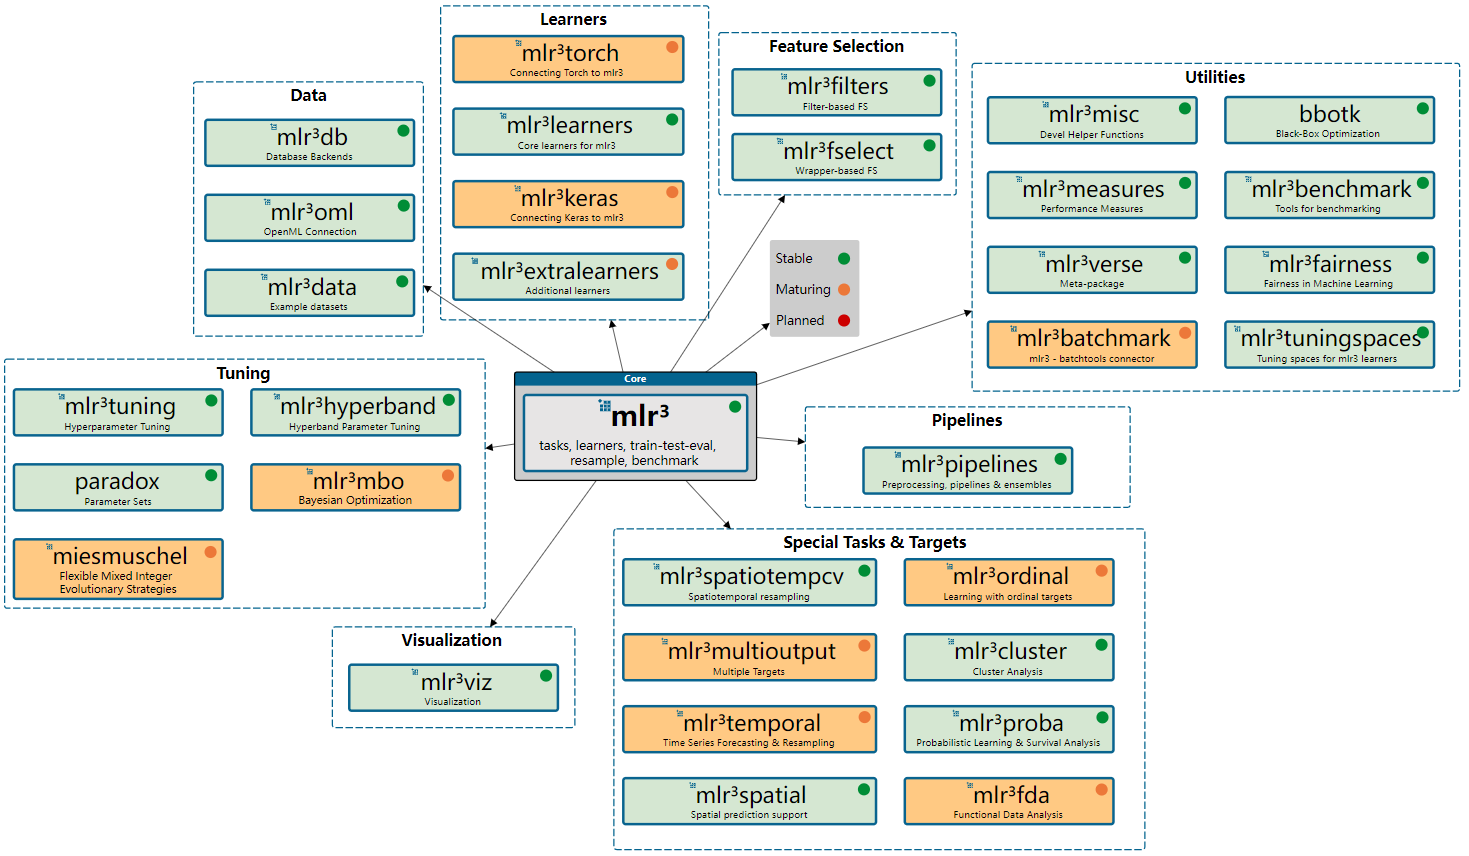
\includegraphics[width=1\linewidth]{images/mlr3_eco} 

}

\caption{mlr3verse生态}\label{fig:unnamed-chunk-5}
\end{figure}
\end{frame}

\begin{frame}[fragile]{二. 基础知识}
\protect\hypertarget{ux4e8c.-ux57faux7840ux77e5ux8bc6}{}
\begin{block}{1. \texttt{R6}类:面向对象}
\protect\hypertarget{r6ux7c7bux9762ux5411ux5bf9ux8c61}{}
支持继承、引用语法,将数据、方法绑定到一个对象。

\begin{figure}

{\centering 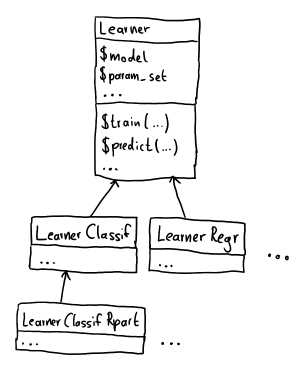
\includegraphics[width=0.4\linewidth]{images/learner_object} 

}

\caption{学习器对象}\label{fig:unnamed-chunk-6}
\end{figure}
\end{block}
\end{frame}

\begin{frame}[fragile]{2. 任务:封装数据}
\protect\hypertarget{ux4efbux52a1ux5c01ux88c5ux6570ux636e}{}
任务是对表格数据的封装,自变量称为特征,因变量称为目标或结果变量。

\begin{itemize}
\tightlist
\item
  目标决定了机器学习的``任务'':

  \begin{itemize}
  \tightlist
  \item
    连续目标,就是回归;
  \item
    离散目标,就是分类;
  \item
    无目标,无监督学习(聚类、降维)
  \end{itemize}
\end{itemize}

\texttt{mlr3}生态下还有若干特殊任务:生存分析任务、密度估计任务、时空分析任务、有序分析任务、函数分析任务、多标签分类任务、成本敏感分类任务、聚类任务。
\end{frame}

\begin{frame}[fragile]{}
\protect\hypertarget{section-2}{}
\begin{itemize}
\tightlist
\item
  创建任务:
\end{itemize}

\begin{Shaded}
\begin{Highlighting}[]
\NormalTok{dat }\OtherTok{=} \FunctionTok{tsk}\NormalTok{(}\StringTok{"german\_credit"}\NormalTok{)}\SpecialCharTok{$}\FunctionTok{data}\NormalTok{()}
\NormalTok{task }\OtherTok{=} \FunctionTok{as\_task\_classif}\NormalTok{(dat, }\AttributeTok{target =} \StringTok{"credit\_risk"}\NormalTok{)}
\NormalTok{task}
\CommentTok{\#\textgreater{} \textless{}TaskClassif:dat\textgreater{} (1000 x 21)}
\CommentTok{\#\textgreater{} * Target: credit\_risk}
\CommentTok{\#\textgreater{} * Properties: twoclass}
\CommentTok{\#\textgreater{} * Features (20):}
\CommentTok{\#\textgreater{}   {-} fct (14): credit\_history, employment\_duration, foreign\_worker,}
\CommentTok{\#\textgreater{}     housing, job, other\_debtors, other\_installment\_plans,}
\CommentTok{\#\textgreater{}     people\_liable, personal\_status\_sex, property, purpose, savings,}
\CommentTok{\#\textgreater{}     status, telephone}
\CommentTok{\#\textgreater{}   {-} int (3): age, amount, duration}
\CommentTok{\#\textgreater{}   {-} ord (3): installment\_rate, number\_credits, present\_residence}
\end{Highlighting}
\end{Shaded}
\end{frame}

\begin{frame}[fragile]{}
\protect\hypertarget{section-3}{}
\begin{itemize}
\tightlist
\item
  若不想使用全部特征
\end{itemize}

\begin{Shaded}
\begin{Highlighting}[]
\NormalTok{task}\SpecialCharTok{$}\FunctionTok{select}\NormalTok{(}\AttributeTok{cols =} \FunctionTok{setdiff}\NormalTok{(task}\SpecialCharTok{$}\NormalTok{feature\_names, }\StringTok{"telephone"}\NormalTok{))}
\end{Highlighting}
\end{Shaded}

\begin{itemize}
\tightlist
\item
  划分训练集、测试集
\end{itemize}

\begin{Shaded}
\begin{Highlighting}[]
\FunctionTok{set.seed}\NormalTok{(}\DecValTok{1}\NormalTok{)}
\NormalTok{split }\OtherTok{=} \FunctionTok{partition}\NormalTok{(task, }\AttributeTok{ratio =} \FloatTok{0.7}\NormalTok{)  }
\CommentTok{\# 默认stratify = TRUE, 按目标变量分层}
\end{Highlighting}
\end{Shaded}

得到训练集、测试集的索引,分别在\texttt{split\$train、split\$test}中。
\end{frame}

\begin{frame}[fragile]{3. 学习器:封装算法}
\protect\hypertarget{ux5b66ux4e60ux5668ux5c01ux88c5ux7b97ux6cd5}{}
\texttt{mlr3}将算法封装在学习器中,提供了统一的方便接口,算法实现整合自相应的算法包(需要安装)。

\begin{Shaded}
\begin{Highlighting}[]
\CommentTok{\# 选择随机森林分类学习器, 需要ranger包}
\NormalTok{learner }\OtherTok{=} \FunctionTok{lrn}\NormalTok{(}\StringTok{"classif.ranger"}\NormalTok{, }\AttributeTok{num.trees =} \DecValTok{100}\NormalTok{, }
              \AttributeTok{predict\_type =} \StringTok{"prob"}\NormalTok{)}
\NormalTok{learner}
\CommentTok{\#\textgreater{} \textless{}LearnerClassifRanger:classif.ranger\textgreater{}}
\CommentTok{\#\textgreater{} * Model: {-}}
\CommentTok{\#\textgreater{} * Parameters: num.threads=1, num.trees=100}
\CommentTok{\#\textgreater{} * Packages: mlr3, mlr3learners, ranger}
\CommentTok{\#\textgreater{} * Predict Types:  response, [prob]}
\CommentTok{\#\textgreater{} * Feature Types: logical, integer, numeric, character, factor, ordered}
\CommentTok{\#\textgreater{} * Properties: hotstart\_backward, importance, multiclass, oob\_error,}
\CommentTok{\#\textgreater{}   twoclass, weights}
\end{Highlighting}
\end{Shaded}
\end{frame}

\begin{frame}{}
\protect\hypertarget{section-4}{}
\begin{figure}

{\centering 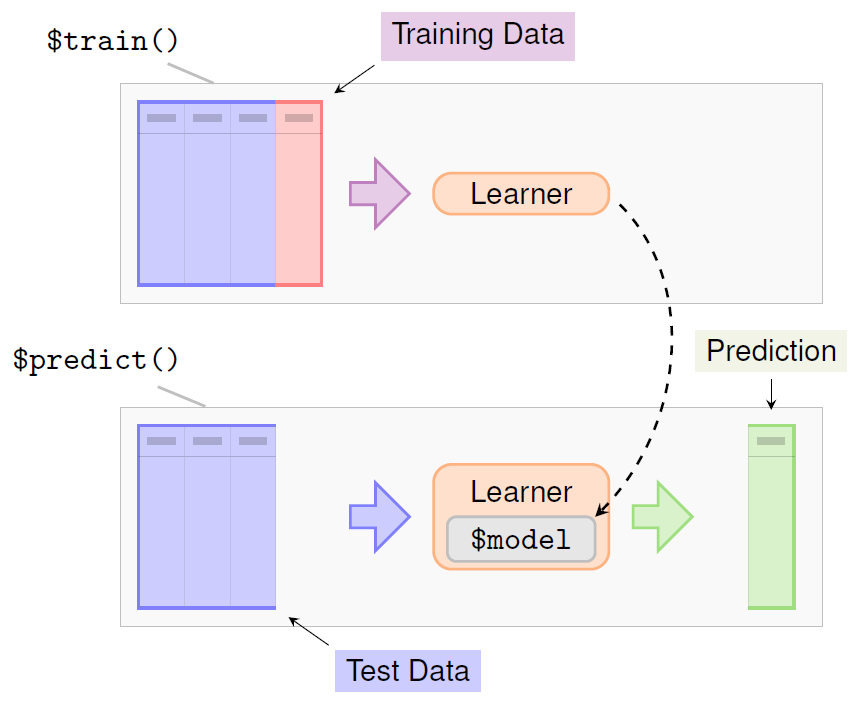
\includegraphics[width=0.75\linewidth]{images/ml_workflow} 

}

\caption{学习器工作流程}\label{fig:unnamed-chunk-11}
\end{figure}
\end{frame}

\begin{frame}[fragile]{}
\protect\hypertarget{section-5}{}
\begin{itemize}
\tightlist
\item
  在训练集上训练模型
\end{itemize}

\begin{Shaded}
\begin{Highlighting}[]
\NormalTok{learner}\SpecialCharTok{$}\FunctionTok{train}\NormalTok{(task, }\AttributeTok{row\_ids =}\NormalTok{ split}\SpecialCharTok{$}\NormalTok{train)}
\NormalTok{learner}\SpecialCharTok{$}\NormalTok{model}
\CommentTok{\#\textgreater{} Ranger result}
\CommentTok{\#\textgreater{} }
\CommentTok{\#\textgreater{} Call:}
\CommentTok{\#\textgreater{}  ranger::ranger(dependent.variable.name = task$target\_names, data = task$data(),      probability = self$predict\_type == "prob", case.weights = task$weights$weight,      num.threads = 1L, num.trees = 100L) }
\CommentTok{\#\textgreater{} }
\CommentTok{\#\textgreater{} Type:                             Probability estimation }
\CommentTok{\#\textgreater{} Number of trees:                  100 }
\CommentTok{\#\textgreater{} Sample size:                      700 }
\CommentTok{\#\textgreater{} Number of independent variables:  19 }
\CommentTok{\#\textgreater{} Mtry:                             4 }
\CommentTok{\#\textgreater{} Target node size:                 10 }
\CommentTok{\#\textgreater{} Variable importance mode:         none }
\CommentTok{\#\textgreater{} Splitrule:                        gini }
\CommentTok{\#\textgreater{} OOB prediction error (Brier s.):  0.162}
\end{Highlighting}
\end{Shaded}
\end{frame}

\begin{frame}[fragile]{}
\protect\hypertarget{section-6}{}
\begin{itemize}
\tightlist
\item
  在测试集上做预测
\end{itemize}

\begin{Shaded}
\begin{Highlighting}[]
\NormalTok{prediction }\OtherTok{=}\NormalTok{ learner}\SpecialCharTok{$}\FunctionTok{predict}\NormalTok{(task, }\AttributeTok{row\_ids =}\NormalTok{ split}\SpecialCharTok{$}\NormalTok{test)}
\NormalTok{prediction}
\CommentTok{\#\textgreater{} \textless{}PredictionClassif\textgreater{} for 300 observations:}
\CommentTok{\#\textgreater{}     row\_ids truth response prob.good prob.bad}
\CommentTok{\#\textgreater{}           8  good     good     0.637   0.3630}
\CommentTok{\#\textgreater{}          15  good     good     0.647   0.3535}
\CommentTok{\#\textgreater{}          17  good     good     1.000   0.0000}
\CommentTok{\#\textgreater{} {-}{-}{-}                                          }
\CommentTok{\#\textgreater{}         979   bad     good     0.924   0.0765}
\CommentTok{\#\textgreater{}         982   bad     good     0.553   0.4468}
\CommentTok{\#\textgreater{}         999   bad      bad     0.306   0.6940}
\end{Highlighting}
\end{Shaded}
\end{frame}

\begin{frame}[fragile]{4. 性能评估}
\protect\hypertarget{ux6027ux80fdux8bc4ux4f30}{}
训练集上训练好的模型性能如何,需要:

\begin{itemize}
\tightlist
\item
  将模型用到测试集得到预测值;
\item
  选择一种合适的性能度量指标,来度量预测值与真实值相差多少。
\end{itemize}

\begin{Shaded}
\begin{Highlighting}[]
\NormalTok{prediction}\SpecialCharTok{$}\FunctionTok{score}\NormalTok{(}\FunctionTok{msr}\NormalTok{(}\StringTok{"classif.acc"}\NormalTok{))   }\CommentTok{\# 准确率}
\CommentTok{\#\textgreater{} classif.acc }
\CommentTok{\#\textgreater{}       0.707}
\NormalTok{prediction}\SpecialCharTok{$}\FunctionTok{score}\NormalTok{(}\FunctionTok{msr}\NormalTok{(}\StringTok{"classif.auc"}\NormalTok{))   }\CommentTok{\# AUC面积}
\CommentTok{\#\textgreater{} classif.auc }
\CommentTok{\#\textgreater{}       0.749}
\end{Highlighting}
\end{Shaded}
\end{frame}

\begin{frame}[fragile]{}
\protect\hypertarget{section-7}{}
\begin{Shaded}
\begin{Highlighting}[]
\CommentTok{\# 绘制ROC曲线, 需要precrec包}
\FunctionTok{autoplot}\NormalTok{(prediction, }\AttributeTok{type =} \StringTok{"roc"}\NormalTok{)     }
\end{Highlighting}
\end{Shaded}

\begin{center}\includegraphics[width=0.78\linewidth]{mlr3workflow_files/figure-beamer/unnamed-chunk-15-1} \end{center}
\end{frame}

\begin{frame}{5. 重抽样}
\protect\hypertarget{ux91cdux62bdux6837}{}
\textbf{重抽样}就是对数据集重复抽样,得到数据集的若干副本。

机器学习传统的数据划分:训练集+测试集,就是对数据的一种重抽样:\textbf{留出法}(``holdout'')。

留出法最简单,只得到了数据集的一个副本,所以只能做一次``拟合模型+模型预测+评估性能''。

从数据集抽样出多个副本,以做多次``拟合模型+模型预测+评估性能'',取平均性能作为最终性能。比如,\textbf{\(k\)折交叉验证}(``cv'')
\end{frame}

\begin{frame}{}
\protect\hypertarget{section-8}{}
\begin{figure}

{\centering 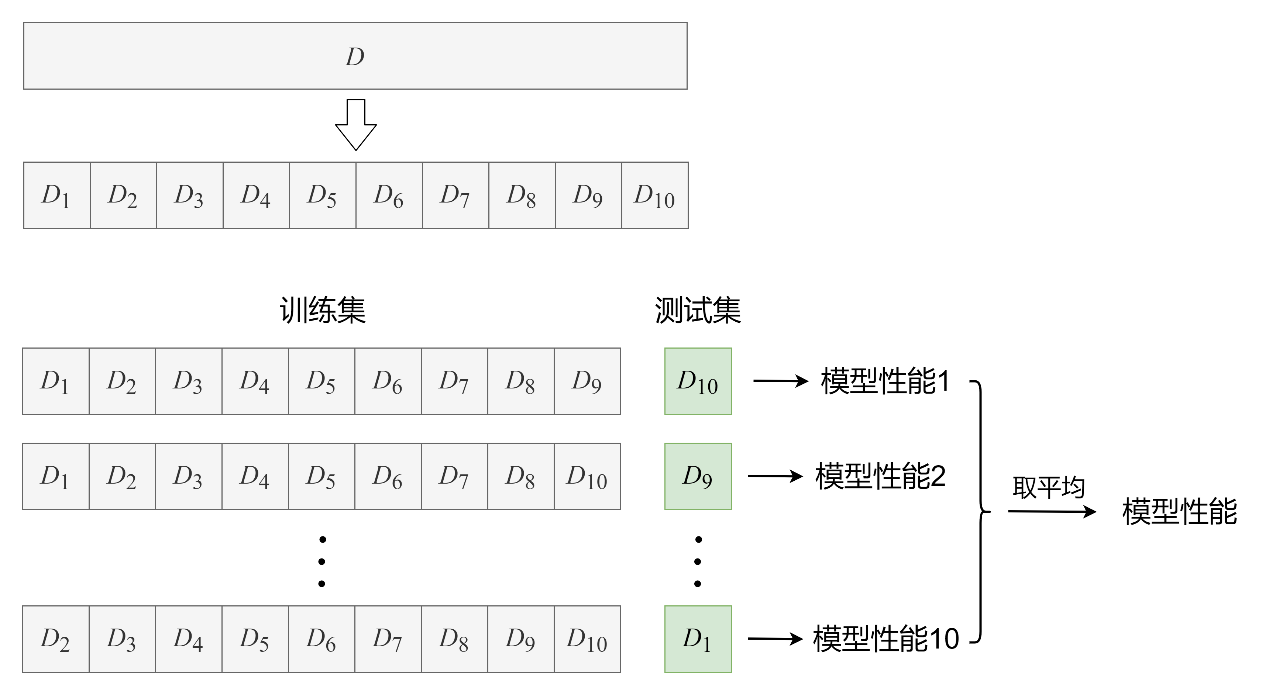
\includegraphics[width=0.9\linewidth]{images/k_folds} 

}

\caption{10折交叉验证}\label{fig:unnamed-chunk-16}
\end{figure}
\end{frame}

\begin{frame}[fragile]{}
\protect\hypertarget{section-9}{}
\begin{itemize}
\tightlist
\item
  使用重抽样
\end{itemize}

\begin{Shaded}
\begin{Highlighting}[]
\NormalTok{cv5 }\OtherTok{=} \FunctionTok{rsmp}\NormalTok{(}\StringTok{"cv"}\NormalTok{, }\AttributeTok{folds =} \DecValTok{5}\NormalTok{)      }\CommentTok{\# 选择重抽样: 5折交叉验证}
\NormalTok{rr }\OtherTok{=} \FunctionTok{resample}\NormalTok{(task, learner, cv5, }\AttributeTok{store\_models =} \ConstantTok{TRUE}\NormalTok{)}
\NormalTok{rr}\SpecialCharTok{$}\FunctionTok{aggregate}\NormalTok{(}\FunctionTok{msr}\NormalTok{(}\StringTok{"classif.acc"}\NormalTok{)) }\CommentTok{\# 所有重抽样的平均准确率}
\CommentTok{\#\textgreater{} classif.acc }
\CommentTok{\#\textgreater{}       0.766}
\NormalTok{rr}\SpecialCharTok{$}\FunctionTok{prediction}\NormalTok{()      }\CommentTok{\# 所有预测合并为一个预测(宏平均)}
\CommentTok{\#\textgreater{} \textless{}PredictionClassif\textgreater{} for 1000 observations:}
\CommentTok{\#\textgreater{}     row\_ids truth response prob.good prob.bad}
\CommentTok{\#\textgreater{}           1  good     good     0.893   0.1074}
\CommentTok{\#\textgreater{}           3  good     good     0.924   0.0758}
\CommentTok{\#\textgreater{}          10   bad     good     0.610   0.3901}
\CommentTok{\#\textgreater{} {-}{-}{-}                                          }
\CommentTok{\#\textgreater{}         987  good      bad     0.415   0.5849}
\CommentTok{\#\textgreater{}         990  good     good     0.731   0.2688}
\CommentTok{\#\textgreater{}         997  good      bad     0.437   0.5629}
\end{Highlighting}
\end{Shaded}
\end{frame}

\begin{frame}[fragile]{}
\protect\hypertarget{section-10}{}
\begin{Shaded}
\begin{Highlighting}[]
\NormalTok{rr}\SpecialCharTok{$}\FunctionTok{score}\NormalTok{(}\FunctionTok{msr}\NormalTok{(}\StringTok{"classif.acc"}\NormalTok{))     }\CommentTok{\# 各个重抽样的准确率}
\CommentTok{\#\textgreater{}                 task task\_id                    learner     learner\_id}
\CommentTok{\#\textgreater{} 1: \textless{}TaskClassif[50]\textgreater{}     dat \textless{}LearnerClassifRanger[38]\textgreater{} classif.ranger}
\CommentTok{\#\textgreater{} 2: \textless{}TaskClassif[50]\textgreater{}     dat \textless{}LearnerClassifRanger[38]\textgreater{} classif.ranger}
\CommentTok{\#\textgreater{} 3: \textless{}TaskClassif[50]\textgreater{}     dat \textless{}LearnerClassifRanger[38]\textgreater{} classif.ranger}
\CommentTok{\#\textgreater{} 4: \textless{}TaskClassif[50]\textgreater{}     dat \textless{}LearnerClassifRanger[38]\textgreater{} classif.ranger}
\CommentTok{\#\textgreater{} 5: \textless{}TaskClassif[50]\textgreater{}     dat \textless{}LearnerClassifRanger[38]\textgreater{} classif.ranger}
\CommentTok{\#\textgreater{}            resampling resampling\_id iteration              prediction}
\CommentTok{\#\textgreater{} 1: \textless{}ResamplingCV[20]\textgreater{}            cv         1 \textless{}PredictionClassif[20]\textgreater{}}
\CommentTok{\#\textgreater{} 2: \textless{}ResamplingCV[20]\textgreater{}            cv         2 \textless{}PredictionClassif[20]\textgreater{}}
\CommentTok{\#\textgreater{} 3: \textless{}ResamplingCV[20]\textgreater{}            cv         3 \textless{}PredictionClassif[20]\textgreater{}}
\CommentTok{\#\textgreater{} 4: \textless{}ResamplingCV[20]\textgreater{}            cv         4 \textless{}PredictionClassif[20]\textgreater{}}
\CommentTok{\#\textgreater{} 5: \textless{}ResamplingCV[20]\textgreater{}            cv         5 \textless{}PredictionClassif[20]\textgreater{}}
\CommentTok{\#\textgreater{}    classif.acc}
\CommentTok{\#\textgreater{} 1:       0.795}
\CommentTok{\#\textgreater{} 2:       0.775}
\CommentTok{\#\textgreater{} 3:       0.770}
\CommentTok{\#\textgreater{} 4:       0.760}
\CommentTok{\#\textgreater{} 5:       0.730}
\end{Highlighting}
\end{Shaded}
\end{frame}

\begin{frame}[fragile]{6. 基准测试}
\protect\hypertarget{ux57faux51c6ux6d4bux8bd5}{}
\textbf{基准测试}(\texttt{benchmark}),用来比较不同学习器(算法)、在多个任务(数据)和/或不同重抽样策略(多个数据副本)上的平均性能表现。

基准测试时有一个关键问题是,测试的公平性,即每个算法的每次测试必须在相同的重抽样训练集拟合模型,在相同的重抽样测试集评估性能。

例如,

\begin{itemize}
\tightlist
\item
  选取一个自带的二分类任务
\item
  选取多个学习器:决策树、\texttt{KNN}、随机森林、支持向量机
\item
  创建基准测试``设计''(每个学习器不能只凭一次结果,采用\(5\)折交叉验证的平均结果)
\item
  查看性能指标:准确率、\texttt{AUC}值
\item
  箱线图展示\texttt{AUC}值的对比结果
\end{itemize}
\end{frame}

\begin{frame}[fragile]{}
\protect\hypertarget{section-11}{}
\begin{Shaded}
\begin{Highlighting}[]
\NormalTok{tasks }\OtherTok{=} \FunctionTok{tsk}\NormalTok{(}\StringTok{"sonar"}\NormalTok{)        }\CommentTok{\# 可以是多个任务}
\NormalTok{learners }\OtherTok{=} \FunctionTok{lrns}\NormalTok{(}\FunctionTok{c}\NormalTok{(}\StringTok{"classif.rpart"}\NormalTok{, }\StringTok{"classif.kknn"}\NormalTok{, }
                  \StringTok{"classif.ranger"}\NormalTok{, }\StringTok{"classif.svm"}\NormalTok{), }
                \AttributeTok{predict\_type =} \StringTok{"prob"}\NormalTok{)}
\NormalTok{design }\OtherTok{=} \FunctionTok{benchmark\_grid}\NormalTok{(tasks, learners, }
                        \FunctionTok{rsmps}\NormalTok{(}\StringTok{"cv"}\NormalTok{, }\AttributeTok{folds =} \DecValTok{5}\NormalTok{))}
\NormalTok{bmr }\OtherTok{=} \FunctionTok{benchmark}\NormalTok{(design)     }\CommentTok{\# 执行基准测试 }
\NormalTok{bmr}\SpecialCharTok{$}\FunctionTok{aggregate}\NormalTok{(}\FunctionTok{list}\NormalTok{(}\FunctionTok{msr}\NormalTok{(}\StringTok{"classif.acc"}\NormalTok{), }\FunctionTok{msr}\NormalTok{(}\StringTok{"classif.auc"}\NormalTok{))) }
\CommentTok{\#\textgreater{}    nr      resample\_result task\_id     learner\_id resampling\_id iters}
\CommentTok{\#\textgreater{} 1:  1 \textless{}ResampleResult[21]\textgreater{}   sonar  classif.rpart            cv     5}
\CommentTok{\#\textgreater{} 2:  2 \textless{}ResampleResult[21]\textgreater{}   sonar   classif.kknn            cv     5}
\CommentTok{\#\textgreater{} 3:  3 \textless{}ResampleResult[21]\textgreater{}   sonar classif.ranger            cv     5}
\CommentTok{\#\textgreater{} 4:  4 \textless{}ResampleResult[21]\textgreater{}   sonar    classif.svm            cv     5}
\CommentTok{\#\textgreater{}    classif.acc classif.auc}
\CommentTok{\#\textgreater{} 1:       0.702       0.743}
\CommentTok{\#\textgreater{} 2:       0.841       0.926}
\CommentTok{\#\textgreater{} 3:       0.807       0.913}
\CommentTok{\#\textgreater{} 4:       0.836       0.923}
\end{Highlighting}
\end{Shaded}
\end{frame}

\begin{frame}[fragile]{}
\protect\hypertarget{section-12}{}
\begin{Shaded}
\begin{Highlighting}[]
\FunctionTok{autoplot}\NormalTok{(bmr, }\AttributeTok{type =} \StringTok{"roc"}\NormalTok{)        }\CommentTok{\# ROC曲线}
\end{Highlighting}
\end{Shaded}

\begin{center}\includegraphics[width=0.78\linewidth]{mlr3workflow_files/figure-beamer/unnamed-chunk-20-1} \end{center}
\end{frame}

\begin{frame}[fragile]{}
\protect\hypertarget{section-13}{}
\begin{Shaded}
\begin{Highlighting}[]
\FunctionTok{autoplot}\NormalTok{(bmr, }\AttributeTok{measure =} \FunctionTok{msr}\NormalTok{(}\StringTok{"classif.auc"}\NormalTok{))  }\CommentTok{\# AUC箱线图}
\end{Highlighting}
\end{Shaded}

\begin{center}\includegraphics[width=0.78\linewidth]{mlr3workflow_files/figure-beamer/unnamed-chunk-21-1} \end{center}
\end{frame}

\begin{frame}[fragile]{三. 图学习器}
\protect\hypertarget{ux4e09.-ux56feux5b66ux4e60ux5668}{}
一个管道运算(\texttt{PipeOp}),表示机器学习管道中的一个计算步骤。一系列的\texttt{PipeOps}通过边连接(\texttt{\%\textgreater{}\textgreater{}\%})构成图(\texttt{Graph}),图可以是简单的线性图,也可以是复杂的非线性图。

这让我们可以像搭建积木一样,搭建出复杂的图,数据将沿着搭建好的图流动,完成从预处理到机器学习算法构成的整个过程:

\begin{itemize}
\tightlist
\item
  选取\texttt{PipeOp},
  通过\texttt{\%\textgreater{}\textgreater{}\%}、\texttt{gunion()}、\texttt{ppl()}等搭建图
\item
  \texttt{Graph\$plot()}绘制图的结构关系;
\item
  \texttt{as\_learner(Graph)}将图转化为学习器,即可跟普通学习器一样使用
\end{itemize}

管道、图学习器主要用于:

\begin{itemize}
\tightlist
\item
  特征工程:缺失值插补、特征变换、特征选择、处理不均衡数据\ldots\ldots{}
\item
  集成学习:装袋法、堆叠法
\item
  分支训练、分块训练
\end{itemize}
\end{frame}

\begin{frame}[fragile]{1. 特征工程}
\protect\hypertarget{ux7279ux5f81ux5de5ux7a0b}{}
机器学习中的数据预处理,也统称为\textbf{特征工程},主要包括:缺失值插补、特征变换,目的是提升模型性能。

\begin{itemize}
\tightlist
\item
  选择特征工程步相应的\texttt{PipeOp};
\item
  多个特征工程步通过管道符\texttt{\%\textgreater{}\textgreater{}\%}连接;
\item
  很多\texttt{PipeOp}都支持\texttt{affect\_columns}参数(接受\texttt{Selector}选择器)
\end{itemize}
\end{frame}

\begin{frame}{}
\protect\hypertarget{section-14}{}
\begin{figure}

{\centering 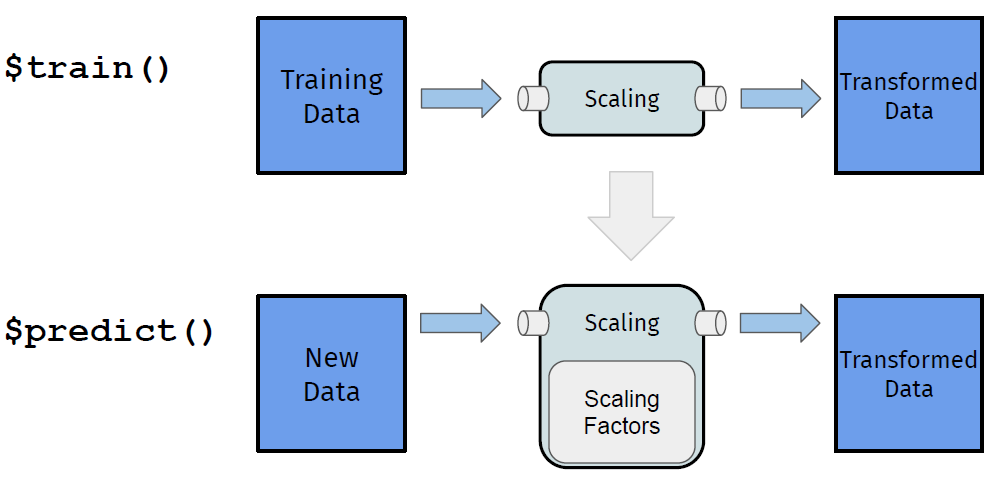
\includegraphics[width=0.75\linewidth]{images/feature_engineering} 

}

\caption{特征工程管道示意图}\label{fig:unnamed-chunk-22}
\end{figure}
\end{frame}

\begin{frame}[fragile]{}
\protect\hypertarget{section-15}{}
\begin{itemize}
\tightlist
\item
  创建特征工程
\end{itemize}

\begin{Shaded}
\begin{Highlighting}[]
\NormalTok{graph }\OtherTok{=} \FunctionTok{po}\NormalTok{(}\StringTok{"scale"}\NormalTok{) }\SpecialCharTok{\%\textgreater{}\textgreater{}\%} \FunctionTok{po}\NormalTok{(}\StringTok{"pca"}\NormalTok{, }\AttributeTok{rank. =} \DecValTok{2}\NormalTok{)}
\NormalTok{graph}\SpecialCharTok{$}\FunctionTok{plot}\NormalTok{()}
\end{Highlighting}
\end{Shaded}

\begin{center}\includegraphics[width=0.78\linewidth]{mlr3workflow_files/figure-beamer/unnamed-chunk-23-1} \end{center}
\end{frame}

\begin{frame}[fragile]{}
\protect\hypertarget{section-16}{}
\begin{itemize}
\tightlist
\item
  \textbf{调试:}查看特征工程对数据做了什么
\end{itemize}

\begin{Shaded}
\begin{Highlighting}[]
\NormalTok{graph}\SpecialCharTok{$}\FunctionTok{train}\NormalTok{(}\FunctionTok{tsk}\NormalTok{(}\StringTok{"iris"}\NormalTok{))[[}\DecValTok{1}\NormalTok{]]}\SpecialCharTok{$}\FunctionTok{data}\NormalTok{()}
\CommentTok{\#\textgreater{}        Species    PC1     PC2}
\CommentTok{\#\textgreater{}   1:    setosa {-}2.257 {-}0.4784}
\CommentTok{\#\textgreater{}   2:    setosa {-}2.074  0.6719}
\CommentTok{\#\textgreater{}   3:    setosa {-}2.356  0.3408}
\CommentTok{\#\textgreater{}   4:    setosa {-}2.292  0.5954}
\CommentTok{\#\textgreater{}   5:    setosa {-}2.382 {-}0.6447}
\CommentTok{\#\textgreater{}  {-}{-}{-}                         }
\CommentTok{\#\textgreater{} 146: virginica  1.864 {-}0.3857}
\CommentTok{\#\textgreater{} 147: virginica  1.559  0.8937}
\CommentTok{\#\textgreater{} 148: virginica  1.516 {-}0.2682}
\CommentTok{\#\textgreater{} 149: virginica  1.368 {-}1.0079}
\CommentTok{\#\textgreater{} 150: virginica  0.957  0.0243}
\end{Highlighting}
\end{Shaded}
\end{frame}

\begin{frame}[fragile]{}
\protect\hypertarget{section-17}{}
\begin{itemize}
\tightlist
\item
  将特征工程用于新数据
\end{itemize}

\begin{Shaded}
\begin{Highlighting}[]
\NormalTok{graph}\SpecialCharTok{$}\FunctionTok{predict}\NormalTok{(}\FunctionTok{tsk}\NormalTok{(}\StringTok{"iris"}\NormalTok{)}\SpecialCharTok{$}\FunctionTok{filter}\NormalTok{(}\DecValTok{1}\SpecialCharTok{:}\DecValTok{5}\NormalTok{))[[}\DecValTok{1}\NormalTok{]]}\SpecialCharTok{$}\FunctionTok{data}\NormalTok{()}
\CommentTok{\#\textgreater{}    Species   PC1    PC2}
\CommentTok{\#\textgreater{} 1:  setosa {-}2.26 {-}0.478}
\CommentTok{\#\textgreater{} 2:  setosa {-}2.07  0.672}
\CommentTok{\#\textgreater{} 3:  setosa {-}2.36  0.341}
\CommentTok{\#\textgreater{} 4:  setosa {-}2.29  0.595}
\CommentTok{\#\textgreater{} 5:  setosa {-}2.38 {-}0.645}
\end{Highlighting}
\end{Shaded}
\end{frame}

\begin{frame}[fragile]{}
\protect\hypertarget{section-18}{}
\begin{itemize}
\tightlist
\item
  \textbf{用于机器学习:}再接一个学习器,转化成图学习器
\end{itemize}

\begin{Shaded}
\begin{Highlighting}[]
\NormalTok{graph }\OtherTok{=}\NormalTok{ graph }\SpecialCharTok{\%\textgreater{}\textgreater{}\%} \FunctionTok{lrn}\NormalTok{(}\StringTok{"classif.rpart"}\NormalTok{)}
\NormalTok{glrn }\OtherTok{=} \FunctionTok{as\_learner}\NormalTok{(graph)}
\end{Highlighting}
\end{Shaded}
\end{frame}

\begin{frame}[fragile]{}
\protect\hypertarget{section-19}{}
\begin{itemize}
\tightlist
\item
  因子特征编码
\end{itemize}

\begin{Shaded}
\begin{Highlighting}[]
\NormalTok{task }\OtherTok{=} \FunctionTok{tsk}\NormalTok{(}\StringTok{"penguins"}\NormalTok{)}
\NormalTok{poe }\OtherTok{=} \FunctionTok{po}\NormalTok{(}\StringTok{"encode"}\NormalTok{, }\AttributeTok{method =} \StringTok{"one{-}hot"}\NormalTok{)    }\CommentTok{\# 独热编码}
\NormalTok{poe}\SpecialCharTok{$}\FunctionTok{train}\NormalTok{(}\FunctionTok{list}\NormalTok{(task))[[}\DecValTok{1}\NormalTok{]]}\SpecialCharTok{$}\FunctionTok{data}\NormalTok{()}
\end{Highlighting}
\end{Shaded}

更多特征工程实现,请参阅\href{https://gitee.com/zhjx19/rconf15}{《R机器学习:mlr3verse技术手册》}\citep{mlr3manual}。
\end{frame}

\begin{frame}{2. 缺失值插补}
\protect\hypertarget{ux7f3aux5931ux503cux63d2ux8865}{}
\begin{itemize}
\tightlist
\item
  缺失值插补,目前支持

  \begin{itemize}
  \tightlist
  \item
    常数、均值、中位数、众数插补
  \item
    随机抽样插补
  \item
    直方图法插补
  \item
    学习器插补
  \item
    超出范围插补
  \item
    增加是否缺失指示列
  \end{itemize}
\end{itemize}
\end{frame}

\begin{frame}[fragile]{}
\protect\hypertarget{section-20}{}
\begin{Shaded}
\begin{Highlighting}[]
\NormalTok{task }\OtherTok{=} \FunctionTok{tsk}\NormalTok{(}\StringTok{"pima"}\NormalTok{)}
\NormalTok{task}\SpecialCharTok{$}\FunctionTok{missings}\NormalTok{()}
\CommentTok{\#\textgreater{} diabetes      age  glucose  insulin     mass pedigree pregnant pressure }
\CommentTok{\#\textgreater{}        0        0        5      374       11        0        0       35 }
\CommentTok{\#\textgreater{}  triceps }
\CommentTok{\#\textgreater{}      227}
\NormalTok{po }\OtherTok{=} \FunctionTok{po}\NormalTok{(}\StringTok{"imputehist"}\NormalTok{)}
\NormalTok{task }\OtherTok{=}\NormalTok{ po}\SpecialCharTok{$}\FunctionTok{train}\NormalTok{(}\FunctionTok{list}\NormalTok{(}\AttributeTok{task =}\NormalTok{ task))[[}\DecValTok{1}\NormalTok{]]}
\NormalTok{task}\SpecialCharTok{$}\FunctionTok{missings}\NormalTok{()}
\CommentTok{\#\textgreater{} diabetes      age pedigree pregnant  glucose  insulin     mass pressure }
\CommentTok{\#\textgreater{}        0        0        0        0        0        0        0        0 }
\CommentTok{\#\textgreater{}  triceps }
\CommentTok{\#\textgreater{}        0}
\end{Highlighting}
\end{Shaded}
\end{frame}

\begin{frame}[fragile]{3. 集成学习}
\protect\hypertarget{ux96c6ux6210ux5b66ux4e60}{}
\begin{itemize}
\tightlist
\item
  \textbf{装袋法(Bagging)}
\end{itemize}

用``有放回''抽样(\texttt{Bootstrap}法)的方式,对包含\(m\)个样本的训练集,进行\(m\)次有放回的随机抽样操作,得到样本子集(有重复)中有接近\(36.8\%\)的样本没有被抽到。按照同样的方式重复进行,就可以采集到\(T\)个包含\(m\)个样本的数据副本,从而训练出\(T\)个基学习器。最终对这\(T\)个基学习器的输出进行结合,分类问题就采用``多数决'',回归问题就采用``取平均''。

\begin{figure}

{\centering 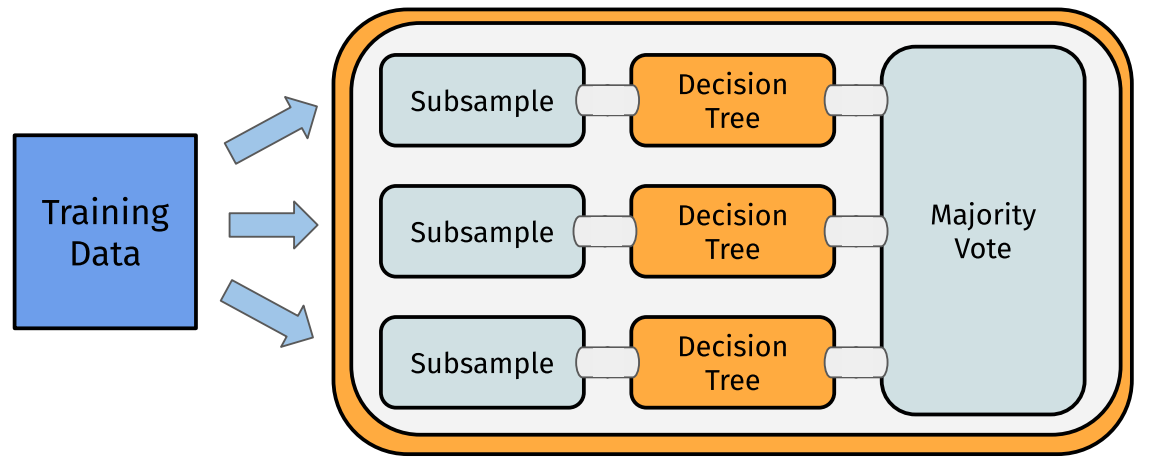
\includegraphics[width=0.7\linewidth]{images/bagging} 

}

\caption{Bagging法管道示意图}\label{fig:unnamed-chunk-29}
\end{figure}
\end{frame}

\begin{frame}[fragile]{}
\protect\hypertarget{section-21}{}
\begin{Shaded}
\begin{Highlighting}[]
\CommentTok{\# 单分支: 数据子抽样+决策树}
\NormalTok{single\_path }\OtherTok{=} \FunctionTok{po}\NormalTok{(}\StringTok{"subsample"}\NormalTok{) }\SpecialCharTok{\%\textgreater{}\textgreater{}\%} \FunctionTok{lrn}\NormalTok{(}\StringTok{"classif.rpart"}\NormalTok{)}
\CommentTok{\# 复制10次得到10个分支, 再接类平均}
\NormalTok{graph\_bag }\OtherTok{=} \FunctionTok{ppl}\NormalTok{(}\StringTok{"greplicate"}\NormalTok{, single\_path, }\AttributeTok{n =} \DecValTok{10}\NormalTok{) }\SpecialCharTok{\%\textgreater{}\textgreater{}\%}
  \FunctionTok{po}\NormalTok{(}\StringTok{"classifavg"}\NormalTok{) }
\end{Highlighting}
\end{Shaded}
\end{frame}

\begin{frame}[fragile]{}
\protect\hypertarget{section-22}{}
\begin{Shaded}
\begin{Highlighting}[]
\NormalTok{graph\_bag}\SpecialCharTok{$}\FunctionTok{plot}\NormalTok{()}
\end{Highlighting}
\end{Shaded}

\begin{center}\includegraphics[width=0.85\linewidth]{mlr3workflow_files/figure-beamer/unnamed-chunk-31-1} \end{center}
\end{frame}

\begin{frame}{}
\protect\hypertarget{section-23}{}
\begin{itemize}
\tightlist
\item
  \textbf{堆叠法(Stacking)}
\end{itemize}

通常采用\(k\)折交叉训练法(类似\(k\)
折交叉验证):每个基学习器分别在各个\(k-1\)
折数据上训练,在其剩下的\(1\)折数据上预测,就可以得到对任意\(1\)折数据的预测结果特征,进而用于训练主模型。

\begin{figure}

{\centering 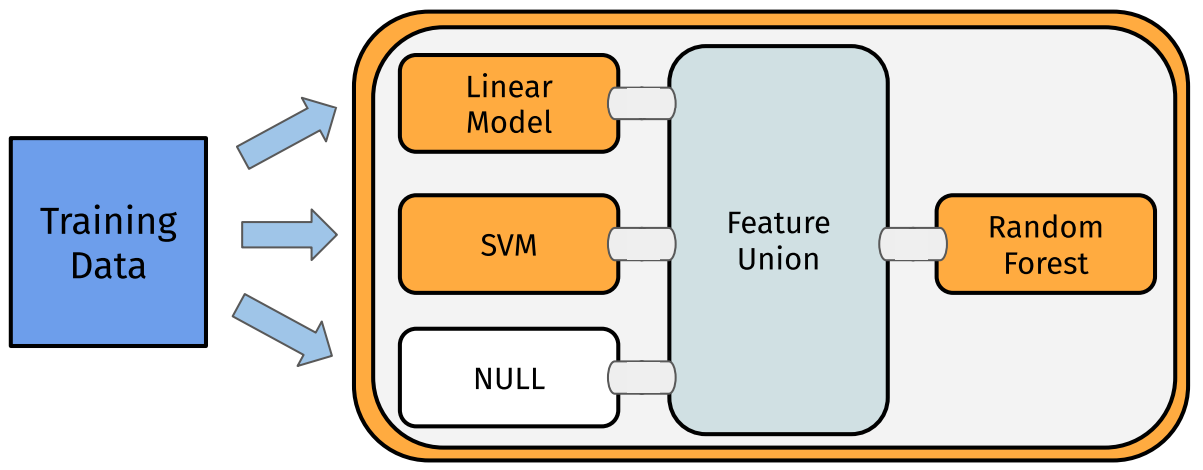
\includegraphics[width=0.65\linewidth]{images/stacking} 

}

\caption{Stacking法管道示意图}\label{fig:unnamed-chunk-32}
\end{figure}
\end{frame}

\begin{frame}[fragile]{}
\protect\hypertarget{section-24}{}
\begin{Shaded}
\begin{Highlighting}[]
\NormalTok{graph\_stack }\OtherTok{=} \FunctionTok{gunion}\NormalTok{(}\FunctionTok{list}\NormalTok{(}
    \FunctionTok{po}\NormalTok{(}\StringTok{"learner\_cv"}\NormalTok{, }\FunctionTok{lrn}\NormalTok{(}\StringTok{"regr.lm"}\NormalTok{)),}
    \FunctionTok{po}\NormalTok{(}\StringTok{"learner\_cv"}\NormalTok{, }\FunctionTok{lrn}\NormalTok{(}\StringTok{"regr.svm"}\NormalTok{)),}
    \FunctionTok{po}\NormalTok{(}\StringTok{"nop"}\NormalTok{))) }\SpecialCharTok{\%\textgreater{}\textgreater{}\%}
  \FunctionTok{po}\NormalTok{(}\StringTok{"featureunion"}\NormalTok{) }\SpecialCharTok{\%\textgreater{}\textgreater{}\%}
  \FunctionTok{lrn}\NormalTok{(}\StringTok{"regr.ranger"}\NormalTok{)}
\end{Highlighting}
\end{Shaded}
\end{frame}

\begin{frame}[fragile]{}
\protect\hypertarget{section-25}{}
\begin{Shaded}
\begin{Highlighting}[]
\NormalTok{graph\_stack}\SpecialCharTok{$}\FunctionTok{plot}\NormalTok{()}
\end{Highlighting}
\end{Shaded}

\begin{center}\includegraphics[width=0.85\linewidth]{mlr3workflow_files/figure-beamer/unnamed-chunk-34-1} \end{center}
\end{frame}

\begin{frame}[fragile]{4. 处理不均衡数据}
\protect\hypertarget{ux5904ux7406ux4e0dux5747ux8861ux6570ux636e}{}
在训练阶段,通过采样对任务进行类平衡,有利于不平衡的数据分类:

\begin{itemize}
\tightlist
\item
  \textbf{欠采样}:只保留多数类的一部分行;
\item
  \textbf{过采样}:对少数类进行超量采样(重复数据点);
\item
  \textbf{SMOTE法}:基于少数类观测的\(K\)个最近邻居生成新观测,只能用于纯数值特征的任务。
\end{itemize}

\begin{Shaded}
\begin{Highlighting}[]
\NormalTok{task }\OtherTok{=} \FunctionTok{tsk}\NormalTok{(}\StringTok{"german\_credit"}\NormalTok{)}
\FunctionTok{table}\NormalTok{(task}\SpecialCharTok{$}\FunctionTok{truth}\NormalTok{())}
\CommentTok{\#\textgreater{} }
\CommentTok{\#\textgreater{} good  bad }
\CommentTok{\#\textgreater{}  700  300}
\end{Highlighting}
\end{Shaded}
\end{frame}

\begin{frame}[fragile]{}
\protect\hypertarget{section-26}{}
\begin{Shaded}
\begin{Highlighting}[]
\CommentTok{\# 只支持double型特征, 需安装smotefamily包}
\NormalTok{pop }\OtherTok{=}  \FunctionTok{po}\NormalTok{(}\StringTok{"colapply"}\NormalTok{, }\AttributeTok{applicator =}\NormalTok{ as.numeric,}
          \AttributeTok{affect\_columns =} \FunctionTok{selector\_type}\NormalTok{(}\StringTok{"integer"}\NormalTok{)) }\SpecialCharTok{\%\textgreater{}\textgreater{}\%}
  \FunctionTok{po}\NormalTok{(}\StringTok{"encodeimpact"}\NormalTok{) }\SpecialCharTok{\%\textgreater{}\textgreater{}\%} 
  \FunctionTok{po}\NormalTok{(}\StringTok{"smote"}\NormalTok{, }\AttributeTok{K =} \DecValTok{5}\NormalTok{, }\AttributeTok{dup\_size =} \DecValTok{1}\NormalTok{)   }\CommentTok{\# 少数类增加1倍}
\NormalTok{result }\OtherTok{=}\NormalTok{ pop}\SpecialCharTok{$}\FunctionTok{train}\NormalTok{(task)[[}\DecValTok{1}\NormalTok{]]}
\FunctionTok{table}\NormalTok{(result}\SpecialCharTok{$}\FunctionTok{truth}\NormalTok{())}
\CommentTok{\#\textgreater{} }
\CommentTok{\#\textgreater{} good  bad }
\CommentTok{\#\textgreater{}  700  600}
\end{Highlighting}
\end{Shaded}
\end{frame}

\begin{frame}[fragile]{5. 分块训练}
\protect\hypertarget{ux5206ux5757ux8badux7ec3}{}
\begin{itemize}
\tightlist
\item
  对无法载入内存的数据,采用分块训练合并模型结果:
\end{itemize}

\begin{Shaded}
\begin{Highlighting}[]
\NormalTok{graph\_chunks }\OtherTok{=} \FunctionTok{po}\NormalTok{(}\StringTok{"chunk"}\NormalTok{, }\DecValTok{4}\NormalTok{) }\SpecialCharTok{\%\textgreater{}\textgreater{}\%}
  \FunctionTok{ppl}\NormalTok{(}\StringTok{"greplicate"}\NormalTok{, }\FunctionTok{lrn}\NormalTok{(}\StringTok{"classif.rpart"}\NormalTok{), }\DecValTok{4}\NormalTok{) }\SpecialCharTok{\%\textgreater{}\textgreater{}\%}
  \FunctionTok{po}\NormalTok{(}\StringTok{"classifavg"}\NormalTok{, }\DecValTok{4}\NormalTok{)}
\end{Highlighting}
\end{Shaded}
\end{frame}

\begin{frame}[fragile]{}
\protect\hypertarget{section-27}{}
\begin{Shaded}
\begin{Highlighting}[]
\NormalTok{graph\_chunks}\SpecialCharTok{$}\FunctionTok{plot}\NormalTok{()}
\end{Highlighting}
\end{Shaded}

\begin{center}\includegraphics[width=0.85\linewidth]{mlr3workflow_files/figure-beamer/unnamed-chunk-38-1} \end{center}
\end{frame}

\begin{frame}{四. 嵌套重抽样}
\protect\hypertarget{ux56db.-ux5d4cux5957ux91cdux62bdux6837}{}
构建模型,是如何从一组潜在的候选模型(如不同的算法,不同的超参数,不同的特征子集)中选择最佳模型。在构建模型过程中所使用的重抽样划分,不应该原样用来评估最终选择模型的性能。

通过在相同的测试集或相同的CV划分上反复评估学习器,测试集的信息会``泄露''到评估中,导致最终的性能估计偏于乐观。

模型构建的所有部分(包括模型选择、预处理)都应该纳入到训练数据的模型寻找过程中。测试集应该只使用一次,测试集只有在模型完全训练好之后才能被使用,例如已确定好了超参数。这样从测试集获得的性能才是真实性能的无偏估计。

对于本身需要重抽样的步骤(如超参数调参),这需要两个嵌套的重抽样循环,即内层调参和外层评估都需要重抽样策略。
\end{frame}

\begin{frame}[fragile]{}
\protect\hypertarget{section-28}{}
嵌套重抽样,即两层重抽样,相当于是两层\texttt{for}循环:

\begin{figure}

{\centering 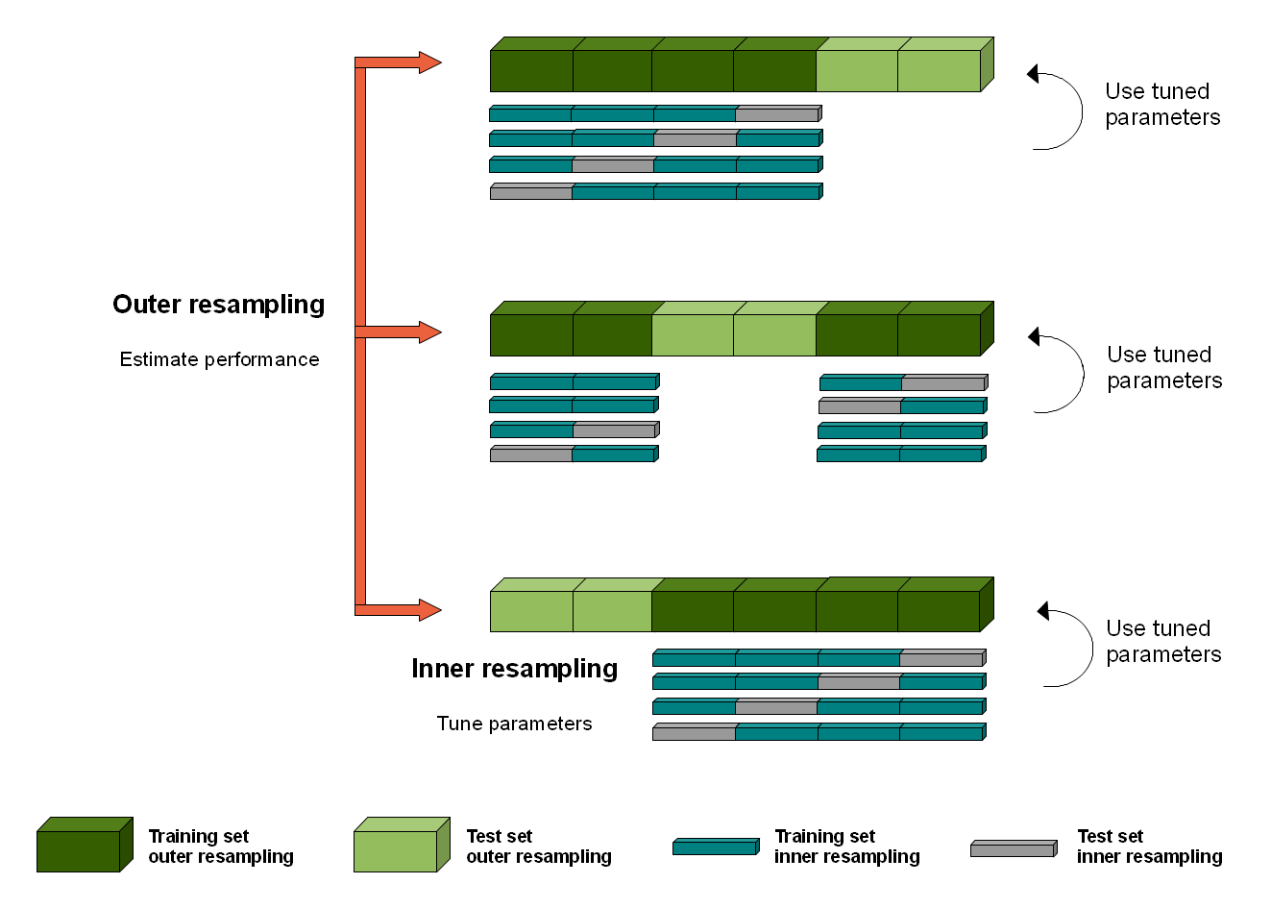
\includegraphics[width=0.78\linewidth]{images/nested_resampling} 

}

\caption{嵌套重抽样示意图}\label{fig:unnamed-chunk-39}
\end{figure}
\end{frame}

\begin{frame}{}
\protect\hypertarget{section-29}{}
\begin{itemize}
\item
  外层是对整个数据集重抽样,\textbf{生成整个数据集的若干副本},每个副本都划分为两部分:\textbf{非测试集}和\textbf{测试集},于是就得到若干组非测试集和测试集划分,用于整体上进行外循环的多次迭代:``在非测试集上做特征选择/超参数调参
  +
  拟合最优特征子集/超参数模型''(也即一轮内循环所做的事情)和``在测试集上评估最优超参数模型性能'',取平均性能作为整个模型的最终性能;
\item
  内层是对每一次外循环的非测试集重抽样,\textbf{生成非测试集的若干副本},每个副本都划分为两部分:\textbf{训练集}和\textbf{验证集},于是就得到若干组训练集(拟合模型)和验证集(评估模型性能)划分,通常是用于做特征选择/超参数调参的内循环多次迭代,以选出最优的特征子集/超参数,确定该次外循环迭代的最优超参数模型;另外,内循环也可用于监视训练过程是否过拟合。
\end{itemize}
\end{frame}

\begin{frame}{}
\protect\hypertarget{section-30}{}
\textbf{注1:}外层每次迭代,都是使用内层重抽样选出最优超参数或特征子集,在整个非测试集上重新训练模型,再在测试集上评估模型性能。

\textbf{注2:}留出(``holdout'')重抽样,只生成数据的\(1\)个副本,无论用于外层或内层,都相当于只循环迭代\(1\)次。
\end{frame}

\begin{frame}[fragile]{五. 超参数调参}
\protect\hypertarget{ux4e94.-ux8d85ux53c2ux6570ux8c03ux53c2}{}
机器学习的模型参数是模型的一阶(直接)参数,是训练模型时用梯度下降法寻优的参数,比如正则化回归模型的回归系数;而超参数是模型的二阶参数,需要事先设定为某值,才能开始训练一阶模型参数,比如正则化回归模型的惩罚参数、\texttt{KNN}的邻居数等。

超参数会对所训练模型的性能产生重大影响,所以不能是(凭经验)随便指定,而是需要设定很多种备选配置,从中选出让模型性能最优的超参数配置,这就是\textbf{超参数调参}。

超参数调参是一项多方联动的系统工作,需要设定:搜索空间、学习器、任务、重抽样策略、模型性能度量指标、终止条件。
\end{frame}

\begin{frame}{}
\protect\hypertarget{section-31}{}
\begin{figure}

{\centering 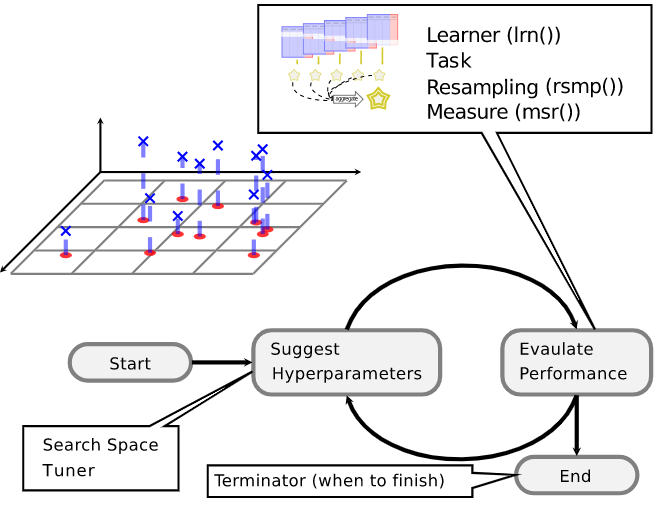
\includegraphics[width=0.75\linewidth]{images/tuning_params} 

}

\caption{超参数调参过程}\label{fig:unnamed-chunk-40}
\end{figure}
\end{frame}

\begin{frame}[fragile]{}
\protect\hypertarget{section-32}{}
超参数调参支持:

\begin{itemize}
\tightlist
\item
  独立调参过程调参:\texttt{tune()}
\item
  自动调参器:\texttt{auto\_tuner()},
  封装成学习器,可用于重抽样或基准测试
\item
  嵌套重抽样调参:\texttt{tune\_nested()}
\end{itemize}

可用\texttt{ps()}创建搜索空间,需提供按类型的调参域构建函数:\texttt{p\_int(),\ p\_dbl(),\ p\_fct(),\ p\_lgl,\ p\_uty()},
其参数有

\begin{itemize}
\tightlist
\item
  \texttt{lower,\ upper}:数值型参数(\texttt{p\_dbl}和\texttt{p\_int})的下限和上限;
\item
  \texttt{levels}:\texttt{p\_fct}参数允许的类别值;
\item
  \texttt{trafo}:变换函数;
\item
  \texttt{depends}:依赖关系。
\end{itemize}
\end{frame}

\begin{frame}[fragile]{}
\protect\hypertarget{section-33}{}
\begin{itemize}
\tightlist
\item
  \textbf{变换}
\end{itemize}

对于数值型超参数,希望当\(x\)均匀变化时,变换后作为超参数能前密后疏。这可以通过\textbf{对数-指数}变换来实现,这也适用于大范围搜索空间。

\begin{Shaded}
\begin{Highlighting}[]
\FunctionTok{library}\NormalTok{(tidyverse)}
\FunctionTok{tibble}\NormalTok{(}\AttributeTok{x =} \DecValTok{1}\SpecialCharTok{:}\DecValTok{20}\NormalTok{,}
       \AttributeTok{y =} \FunctionTok{exp}\NormalTok{(}\FunctionTok{seq}\NormalTok{(}\FunctionTok{log}\NormalTok{(}\DecValTok{3}\NormalTok{), }\FunctionTok{log}\NormalTok{(}\DecValTok{50}\NormalTok{), }\AttributeTok{length.out=}\DecValTok{20}\NormalTok{))) }\SpecialCharTok{\%\textgreater{}\%}
  \FunctionTok{ggplot}\NormalTok{(}\FunctionTok{aes}\NormalTok{(x, y)) }\SpecialCharTok{+} 
  \FunctionTok{geom\_point}\NormalTok{()}
\end{Highlighting}
\end{Shaded}
\end{frame}

\begin{frame}{}
\protect\hypertarget{section-34}{}
\begin{center}\includegraphics[width=0.78\linewidth]{mlr3workflow_files/figure-beamer/unnamed-chunk-42-1} \end{center}
\end{frame}

\begin{frame}[fragile]{}
\protect\hypertarget{section-35}{}
\begin{itemize}
\tightlist
\item
  \textbf{依赖关系}
\end{itemize}

有些超参数只有在另一个参数取某些值时才有意义。例如,支持向量机有一个\texttt{degree}参数,只有在\texttt{kernel}为''polynomial''时才有效。这可以用\texttt{depends}参数来指定:

\begin{Shaded}
\begin{Highlighting}[]
\NormalTok{search\_space }\OtherTok{=} \FunctionTok{ps}\NormalTok{(}
  \AttributeTok{cost =} \FunctionTok{p\_dbl}\NormalTok{(}\FunctionTok{log}\NormalTok{(}\FloatTok{0.1}\NormalTok{), }\FunctionTok{log}\NormalTok{(}\DecValTok{10}\NormalTok{), }
               \AttributeTok{trafo =} \ControlFlowTok{function}\NormalTok{(x) }\FunctionTok{exp}\NormalTok{(x)),}
  \AttributeTok{kernel =} \FunctionTok{p\_fct}\NormalTok{(}\FunctionTok{c}\NormalTok{(}\StringTok{"polynomial"}\NormalTok{, }\StringTok{"radial"}\NormalTok{)),}
  \AttributeTok{degree =} \FunctionTok{p\_int}\NormalTok{(}\DecValTok{1}\NormalTok{, }\DecValTok{3}\NormalTok{, }\AttributeTok{depends =}\NormalTok{ kernel }\SpecialCharTok{==} \StringTok{"polynomial"}\NormalTok{))}
\end{Highlighting}
\end{Shaded}
\end{frame}

\begin{frame}[fragile]{}
\protect\hypertarget{section-36}{}
直接看一个复杂的图学习器嵌套重抽样超参数调参的实例。

图学习器一旦成功创建,就可以像普通学习器一样使用,超参数调参时,原算法的超参数名字都自动带了学习器名字前缀,另外还可以对管道参数调参。

\begin{itemize}
\tightlist
\item
  选取任务
\end{itemize}

\begin{Shaded}
\begin{Highlighting}[]
\NormalTok{task }\OtherTok{=} \FunctionTok{tsk}\NormalTok{(}\StringTok{"pima"}\NormalTok{)}
\end{Highlighting}
\end{Shaded}
\end{frame}

\begin{frame}[fragile]{}
\protect\hypertarget{section-37}{}
\begin{itemize}
\tightlist
\item
  该任务包含缺失值,还有若干因子特征,都需要做预处理:
\end{itemize}

\begin{Shaded}
\begin{Highlighting}[]
\NormalTok{prep }\OtherTok{=} \FunctionTok{gunion}\NormalTok{(}\FunctionTok{list}\NormalTok{(}
    \FunctionTok{po}\NormalTok{(}\StringTok{"imputehist"}\NormalTok{), }
    \FunctionTok{po}\NormalTok{(}\StringTok{"missind"}\NormalTok{, }\AttributeTok{affect\_columns =} 
         \FunctionTok{selector\_type}\NormalTok{(}\FunctionTok{c}\NormalTok{(}\StringTok{"numeric"}\NormalTok{,}\StringTok{"integer"}\NormalTok{))))) }\SpecialCharTok{\%\textgreater{}\textgreater{}\%}
  \FunctionTok{po}\NormalTok{(}\StringTok{"featureunion"}\NormalTok{) }\SpecialCharTok{\%\textgreater{}\textgreater{}\%}
  \FunctionTok{po}\NormalTok{(}\StringTok{"encode"}\NormalTok{) }\SpecialCharTok{\%\textgreater{}\textgreater{}\%}
  \FunctionTok{po}\NormalTok{(}\StringTok{"removeconstants"}\NormalTok{)}
\end{Highlighting}
\end{Shaded}
\end{frame}

\begin{frame}[fragile]{}
\protect\hypertarget{section-38}{}
\begin{itemize}
\tightlist
\item
  选择3个学习器:\texttt{KNN、SVM、Ranger}作为三分支分别拟合模型,再合并分支:
\end{itemize}

\begin{Shaded}
\begin{Highlighting}[]
\NormalTok{learners }\OtherTok{=} \FunctionTok{list}\NormalTok{(}
  \AttributeTok{knn =} \FunctionTok{lrn}\NormalTok{(}\StringTok{"classif.kknn"}\NormalTok{, }\AttributeTok{id =} \StringTok{"kknn"}\NormalTok{),}
  \AttributeTok{svm =} \FunctionTok{lrn}\NormalTok{(}\StringTok{"classif.svm"}\NormalTok{, }\AttributeTok{id =} \StringTok{"svm"}\NormalTok{, }
            \AttributeTok{type =} \StringTok{"C{-}classification"}\NormalTok{),}
  \AttributeTok{rf =} \FunctionTok{lrn}\NormalTok{(}\StringTok{"classif.ranger"}\NormalTok{, }\AttributeTok{id =} \StringTok{"ranger"}\NormalTok{))}
\NormalTok{graph }\OtherTok{=} \FunctionTok{ppl}\NormalTok{(}\StringTok{"branch"}\NormalTok{, learners)}
\end{Highlighting}
\end{Shaded}
\end{frame}

\begin{frame}[fragile]{}
\protect\hypertarget{section-39}{}
\begin{itemize}
\tightlist
\item
  将预处理图和算法图连接得到整个图:
\end{itemize}

\begin{Shaded}
\begin{Highlighting}[]
\NormalTok{graph }\OtherTok{=}\NormalTok{ prep }\SpecialCharTok{\%\textgreater{}\textgreater{}\%}\NormalTok{ graph}
\NormalTok{graph}\SpecialCharTok{$}\FunctionTok{plot}\NormalTok{()}
\end{Highlighting}
\end{Shaded}

\begin{center}\includegraphics[width=0.78\linewidth]{mlr3workflow_files/figure-beamer/unnamed-chunk-47-1} \end{center}
\end{frame}

\begin{frame}[fragile]{}
\protect\hypertarget{section-40}{}
\begin{itemize}
\tightlist
\item
  转化为图学习器,查看其超参数:
\end{itemize}

\begin{Shaded}
\begin{Highlighting}[]
\NormalTok{glearner }\OtherTok{=} \FunctionTok{as\_learner}\NormalTok{(graph)}
\NormalTok{glearner}\SpecialCharTok{$}\NormalTok{param\_set }
\CommentTok{\#\textgreater{} \textless{}ParamSetCollection\textgreater{}}
\CommentTok{\#\textgreater{}                                      id    class lower upper nlevels}
\CommentTok{\#\textgreater{}  1:                    branch.selection ParamFct    NA    NA       3}
\CommentTok{\#\textgreater{}  2:               encode.affect\_columns ParamUty    NA    NA     Inf}
\CommentTok{\#\textgreater{}  3:                       encode.method ParamFct    NA    NA       5}
\CommentTok{\#\textgreater{}  4:           imputehist.affect\_columns ParamUty    NA    NA     Inf}
\CommentTok{\#\textgreater{}  5:                       kknn.distance ParamDbl     0   Inf     Inf}
\CommentTok{\#\textgreater{}  6:                              kknn.k ParamInt     1   Inf     Inf}
\CommentTok{\#\textgreater{}  7:                         kknn.kernel ParamFct    NA    NA      10}
\CommentTok{\#\textgreater{}  8:                          kknn.scale ParamLgl    NA    NA       2}
\CommentTok{\#\textgreater{}  9:                    kknn.store\_model ParamLgl    NA    NA       2}
\CommentTok{\#\textgreater{} 10:                        kknn.ykernel ParamUty    NA    NA     Inf}
\CommentTok{\#\textgreater{} 11:              missind.affect\_columns ParamUty    NA    NA     Inf}
\CommentTok{\#\textgreater{} 12:                        missind.type ParamFct    NA    NA       4}
\CommentTok{\#\textgreater{} 13:                       missind.which ParamFct    NA    NA       2}
\CommentTok{\#\textgreater{} 14:                        ranger.alpha ParamDbl  {-}Inf   Inf     Inf}
\CommentTok{\#\textgreater{} 15:       ranger.always.split.variables ParamUty    NA    NA     Inf}
\CommentTok{\#\textgreater{} 16:                ranger.class.weights ParamUty    NA    NA     Inf}
\CommentTok{\#\textgreater{} 17:                      ranger.holdout ParamLgl    NA    NA       2}
\CommentTok{\#\textgreater{} 18:                   ranger.importance ParamFct    NA    NA       4}
\CommentTok{\#\textgreater{} 19:                   ranger.keep.inbag ParamLgl    NA    NA       2}
\CommentTok{\#\textgreater{} 20:                    ranger.max.depth ParamInt     0   Inf     Inf}
\CommentTok{\#\textgreater{} 21:                ranger.min.node.size ParamInt     1   Inf     Inf}
\CommentTok{\#\textgreater{} 22:                     ranger.min.prop ParamDbl  {-}Inf   Inf     Inf}
\CommentTok{\#\textgreater{} 23:                      ranger.minprop ParamDbl  {-}Inf   Inf     Inf}
\CommentTok{\#\textgreater{} 24:                         ranger.mtry ParamInt     1   Inf     Inf}
\CommentTok{\#\textgreater{} 25:                   ranger.mtry.ratio ParamDbl     0     1     Inf}
\CommentTok{\#\textgreater{} 26:            ranger.num.random.splits ParamInt     1   Inf     Inf}
\CommentTok{\#\textgreater{} 27:                  ranger.num.threads ParamInt     1   Inf     Inf}
\CommentTok{\#\textgreater{} 28:                    ranger.num.trees ParamInt     1   Inf     Inf}
\CommentTok{\#\textgreater{} 29:                    ranger.oob.error ParamLgl    NA    NA       2}
\CommentTok{\#\textgreater{} 30:        ranger.regularization.factor ParamUty    NA    NA     Inf}
\CommentTok{\#\textgreater{} 31:      ranger.regularization.usedepth ParamLgl    NA    NA       2}
\CommentTok{\#\textgreater{} 32:                      ranger.replace ParamLgl    NA    NA       2}
\CommentTok{\#\textgreater{} 33:    ranger.respect.unordered.factors ParamFct    NA    NA       3}
\CommentTok{\#\textgreater{} 34:              ranger.sample.fraction ParamDbl     0     1     Inf}
\CommentTok{\#\textgreater{} 35:                  ranger.save.memory ParamLgl    NA    NA       2}
\CommentTok{\#\textgreater{} 36: ranger.scale.permutation.importance ParamLgl    NA    NA       2}
\CommentTok{\#\textgreater{} 37:                    ranger.se.method ParamFct    NA    NA       2}
\CommentTok{\#\textgreater{} 38:                         ranger.seed ParamInt  {-}Inf   Inf     Inf}
\CommentTok{\#\textgreater{} 39:         ranger.split.select.weights ParamUty    NA    NA     Inf}
\CommentTok{\#\textgreater{} 40:                    ranger.splitrule ParamFct    NA    NA       3}
\CommentTok{\#\textgreater{} 41:                      ranger.verbose ParamLgl    NA    NA       2}
\CommentTok{\#\textgreater{} 42:                 ranger.write.forest ParamLgl    NA    NA       2}
\CommentTok{\#\textgreater{} 43:             removeconstants.abs\_tol ParamDbl     0   Inf     Inf}
\CommentTok{\#\textgreater{} 44:      removeconstants.affect\_columns ParamUty    NA    NA     Inf}
\CommentTok{\#\textgreater{} 45:           removeconstants.na\_ignore ParamLgl    NA    NA       2}
\CommentTok{\#\textgreater{} 46:               removeconstants.ratio ParamDbl     0     1     Inf}
\CommentTok{\#\textgreater{} 47:             removeconstants.rel\_tol ParamDbl     0   Inf     Inf}
\CommentTok{\#\textgreater{} 48:                       svm.cachesize ParamDbl  {-}Inf   Inf     Inf}
\CommentTok{\#\textgreater{} 49:                   svm.class.weights ParamUty    NA    NA     Inf}
\CommentTok{\#\textgreater{} 50:                           svm.coef0 ParamDbl  {-}Inf   Inf     Inf}
\CommentTok{\#\textgreater{} 51:                            svm.cost ParamDbl     0   Inf     Inf}
\CommentTok{\#\textgreater{} 52:                           svm.cross ParamInt     0   Inf     Inf}
\CommentTok{\#\textgreater{} 53:                 svm.decision.values ParamLgl    NA    NA       2}
\CommentTok{\#\textgreater{} 54:                          svm.degree ParamInt     1   Inf     Inf}
\CommentTok{\#\textgreater{} 55:                         svm.epsilon ParamDbl     0   Inf     Inf}
\CommentTok{\#\textgreater{} 56:                          svm.fitted ParamLgl    NA    NA       2}
\CommentTok{\#\textgreater{} 57:                           svm.gamma ParamDbl     0   Inf     Inf}
\CommentTok{\#\textgreater{} 58:                          svm.kernel ParamFct    NA    NA       4}
\CommentTok{\#\textgreater{} 59:                              svm.nu ParamDbl  {-}Inf   Inf     Inf}
\CommentTok{\#\textgreater{} 60:                           svm.scale ParamUty    NA    NA     Inf}
\CommentTok{\#\textgreater{} 61:                       svm.shrinking ParamLgl    NA    NA       2}
\CommentTok{\#\textgreater{} 62:                       svm.tolerance ParamDbl     0   Inf     Inf}
\CommentTok{\#\textgreater{} 63:                            svm.type ParamFct    NA    NA       2}
\CommentTok{\#\textgreater{}                                      id    class lower upper nlevels}
\CommentTok{\#\textgreater{}              default           parents            value}
\CommentTok{\#\textgreater{}  1:   \textless{}NoDefault[3]\textgreater{}                                knn}
\CommentTok{\#\textgreater{}  2:    \textless{}Selector[1]\textgreater{}                                   }
\CommentTok{\#\textgreater{}  3:   \textless{}NoDefault[3]\textgreater{}                            one{-}hot}
\CommentTok{\#\textgreater{}  4:   \textless{}NoDefault[3]\textgreater{}                                   }
\CommentTok{\#\textgreater{}  5:                2                                   }
\CommentTok{\#\textgreater{}  6:                7                                  7}
\CommentTok{\#\textgreater{}  7:          optimal                                   }
\CommentTok{\#\textgreater{}  8:             TRUE                                   }
\CommentTok{\#\textgreater{}  9:            FALSE                                   }
\CommentTok{\#\textgreater{} 10:                                                    }
\CommentTok{\#\textgreater{} 11:    \textless{}Selector[1]\textgreater{}                      \textless{}Selector[1]\textgreater{}}
\CommentTok{\#\textgreater{} 12:   \textless{}NoDefault[3]\textgreater{}                             factor}
\CommentTok{\#\textgreater{} 13:   \textless{}NoDefault[3]\textgreater{}                      missing\_train}
\CommentTok{\#\textgreater{} 14:              0.5                                   }
\CommentTok{\#\textgreater{} 15:   \textless{}NoDefault[3]\textgreater{}                                   }
\CommentTok{\#\textgreater{} 16:                                                    }
\CommentTok{\#\textgreater{} 17:            FALSE                                   }
\CommentTok{\#\textgreater{} 18:   \textless{}NoDefault[3]\textgreater{}                                   }
\CommentTok{\#\textgreater{} 19:            FALSE                                   }
\CommentTok{\#\textgreater{} 20:                                                    }
\CommentTok{\#\textgreater{} 21:                                                    }
\CommentTok{\#\textgreater{} 22:              0.1                                   }
\CommentTok{\#\textgreater{} 23:              0.1                                   }
\CommentTok{\#\textgreater{} 24:   \textless{}NoDefault[3]\textgreater{}                                   }
\CommentTok{\#\textgreater{} 25:   \textless{}NoDefault[3]\textgreater{}                                   }
\CommentTok{\#\textgreater{} 26:                1  ranger.splitrule                 }
\CommentTok{\#\textgreater{} 27:                1                                  1}
\CommentTok{\#\textgreater{} 28:              500                                   }
\CommentTok{\#\textgreater{} 29:             TRUE                                   }
\CommentTok{\#\textgreater{} 30:                1                                   }
\CommentTok{\#\textgreater{} 31:            FALSE                                   }
\CommentTok{\#\textgreater{} 32:             TRUE                                   }
\CommentTok{\#\textgreater{} 33:           ignore                                   }
\CommentTok{\#\textgreater{} 34:   \textless{}NoDefault[3]\textgreater{}                                   }
\CommentTok{\#\textgreater{} 35:            FALSE                                   }
\CommentTok{\#\textgreater{} 36:            FALSE ranger.importance                 }
\CommentTok{\#\textgreater{} 37:          infjack                                   }
\CommentTok{\#\textgreater{} 38:                                                    }
\CommentTok{\#\textgreater{} 39:                                                    }
\CommentTok{\#\textgreater{} 40:             gini                                   }
\CommentTok{\#\textgreater{} 41:             TRUE                                   }
\CommentTok{\#\textgreater{} 42:             TRUE                                   }
\CommentTok{\#\textgreater{} 43:   \textless{}NoDefault[3]\textgreater{}                              1e{-}08}
\CommentTok{\#\textgreater{} 44:    \textless{}Selector[1]\textgreater{}                                   }
\CommentTok{\#\textgreater{} 45:   \textless{}NoDefault[3]\textgreater{}                               TRUE}
\CommentTok{\#\textgreater{} 46:   \textless{}NoDefault[3]\textgreater{}                                  0}
\CommentTok{\#\textgreater{} 47:   \textless{}NoDefault[3]\textgreater{}                              1e{-}08}
\CommentTok{\#\textgreater{} 48:               40                                   }
\CommentTok{\#\textgreater{} 49:                                                    }
\CommentTok{\#\textgreater{} 50:                0        svm.kernel                 }
\CommentTok{\#\textgreater{} 51:                1          svm.type                 }
\CommentTok{\#\textgreater{} 52:                0                                   }
\CommentTok{\#\textgreater{} 53:            FALSE                                   }
\CommentTok{\#\textgreater{} 54:                3        svm.kernel                 }
\CommentTok{\#\textgreater{} 55:              0.1                                   }
\CommentTok{\#\textgreater{} 56:             TRUE                                   }
\CommentTok{\#\textgreater{} 57:   \textless{}NoDefault[3]\textgreater{}        svm.kernel                 }
\CommentTok{\#\textgreater{} 58:           radial                                   }
\CommentTok{\#\textgreater{} 59:              0.5          svm.type                 }
\CommentTok{\#\textgreater{} 60:             TRUE                                   }
\CommentTok{\#\textgreater{} 61:             TRUE                                   }
\CommentTok{\#\textgreater{} 62:            0.001                                   }
\CommentTok{\#\textgreater{} 63: C{-}classification                   C{-}classification}
\CommentTok{\#\textgreater{}              default           parents            value}
\end{Highlighting}
\end{Shaded}
\end{frame}

\begin{frame}[fragile]{}
\protect\hypertarget{section-41}{}
\begin{itemize}
\tightlist
\item
  嵌套重抽样超参数调参,为了加速计算,启动并行:
\end{itemize}

\begin{Shaded}
\begin{Highlighting}[]
\CommentTok{\# future::plan("multicore")      \# win系统不支持多核}
\NormalTok{future}\SpecialCharTok{::}\FunctionTok{plan}\NormalTok{(}\StringTok{"multisession"}\NormalTok{)     }\CommentTok{\# 只支持多线程(异步)}
\end{Highlighting}
\end{Shaded}

\begin{itemize}
\tightlist
\item
  设置搜索空间:
\end{itemize}

\begin{Shaded}
\begin{Highlighting}[]
\NormalTok{search\_space }\OtherTok{=} \FunctionTok{ps}\NormalTok{(}
  \AttributeTok{branch.selection =} \FunctionTok{p\_fct}\NormalTok{(}\FunctionTok{c}\NormalTok{(}\StringTok{"kknn"}\NormalTok{, }\StringTok{"svm"}\NormalTok{, }\StringTok{"ranger"}\NormalTok{)),}
  \AttributeTok{kknn.k =} \FunctionTok{p\_int}\NormalTok{(}\DecValTok{3}\NormalTok{, }\DecValTok{50}\NormalTok{, }\AttributeTok{logscale =} \ConstantTok{TRUE}\NormalTok{, }
                 \AttributeTok{depends =}\NormalTok{ branch.selection }\SpecialCharTok{==} \StringTok{"kknn"}\NormalTok{),}
  \AttributeTok{svm.cost =} \FunctionTok{p\_dbl}\NormalTok{(}\SpecialCharTok{{-}}\DecValTok{1}\NormalTok{, }\DecValTok{1}\NormalTok{, }\AttributeTok{trafo =} \ControlFlowTok{function}\NormalTok{(x) }\DecValTok{10}\SpecialCharTok{\^{}}\NormalTok{x, }
                   \AttributeTok{depends =}\NormalTok{ branch.selection }\SpecialCharTok{==} \StringTok{"svm"}\NormalTok{),}
  \AttributeTok{ranger.mtry =} \FunctionTok{p\_int}\NormalTok{(}\DecValTok{1}\NormalTok{, }\DecValTok{8}\NormalTok{, }
                  \AttributeTok{depends =}\NormalTok{ branch.selection }\SpecialCharTok{==} \StringTok{"ranger"}\NormalTok{))}
\end{Highlighting}
\end{Shaded}
\end{frame}

\begin{frame}[fragile]{}
\protect\hypertarget{section-42}{}
\begin{itemize}
\tightlist
\item
  用\texttt{tune\_nested()}做嵌套调参:外层4折交叉验证、内层3折交叉验证
\end{itemize}

\begin{Shaded}
\begin{Highlighting}[]
\NormalTok{rr }\OtherTok{=} \FunctionTok{tune\_nested}\NormalTok{(}
  \AttributeTok{method =} \StringTok{"random\_search"}\NormalTok{,}
  \AttributeTok{task =}\NormalTok{ task,}
  \AttributeTok{learner =}\NormalTok{ glearner,}
  \AttributeTok{inner\_resampling =} \FunctionTok{rsmp}\NormalTok{ (}\StringTok{"cv"}\NormalTok{, }\AttributeTok{folds =} \DecValTok{3}\NormalTok{),}
  \AttributeTok{outer\_resampling =} \FunctionTok{rsmp}\NormalTok{(}\StringTok{"cv"}\NormalTok{, }\AttributeTok{folds =} \DecValTok{4}\NormalTok{),}
  \AttributeTok{measure =} \FunctionTok{msr}\NormalTok{(}\StringTok{"classif.ce"}\NormalTok{),}
  \AttributeTok{term\_evals =} \DecValTok{10}\NormalTok{)}
\end{Highlighting}
\end{Shaded}

\begin{itemize}
\tightlist
\item
  \texttt{method}:
  调参方法,支持''grid\_search''(网格搜索)、``random\_search''(随机搜索)、gensa(广义模拟退火)、``nloptr''(非线性优化)。
\end{itemize}
\end{frame}

\begin{frame}[fragile]{}
\protect\hypertarget{section-43}{}
\begin{itemize}
\tightlist
\item
  查看调参结果
\end{itemize}

\begin{Shaded}
\begin{Highlighting}[]
\NormalTok{rr}\SpecialCharTok{$}\FunctionTok{aggregate}\NormalTok{()    }\CommentTok{\# 总的平均模型性能}
\CommentTok{\#\textgreater{} classif.ce }
\CommentTok{\#\textgreater{}      0.286}
\end{Highlighting}
\end{Shaded}

\begin{Shaded}
\begin{Highlighting}[]
\NormalTok{rr}\SpecialCharTok{$}\FunctionTok{score}\NormalTok{()        }\CommentTok{\# 外层4次迭代每次的模型性能(结果略)}
\FunctionTok{extract\_inner\_tuning\_results}\NormalTok{(rr)   }\CommentTok{\# 内层调参结果(结果略)}
\FunctionTok{extract\_inner\_tuning\_archives}\NormalTok{(rr)  }\CommentTok{\# 内层的调参档案(结果略)}
\end{Highlighting}
\end{Shaded}

另外,还有其它调参包:\texttt{mlr3hyperband}包(基于逐次减半算法的\texttt{multifidelity}优化)、\texttt{mlr3mbo}包(灵活贝叶斯优化)、\texttt{miesmuschel}包(混合整数进化策略)。
\end{frame}

\begin{frame}[fragile]{六. 特征选择}
\protect\hypertarget{ux516d.-ux7279ux5f81ux9009ux62e9}{}
当数据集包含很多特征时,只提取最重要的部分特征来建模,称为特征选择。特征选择可以增强模型的解释性、加速学习过程、改进学习器性能。

\begin{block}{1. 过滤法}
\protect\hypertarget{ux8fc7ux6ee4ux6cd5}{}
\textbf{过滤法},基于某种衡量特征重要度的指标(如相关系数),用外部算法计算变量的排名,只选用排名靠前的若干特征,用\texttt{mlr3filters}包实现。

\begin{enumerate}
[(1)]
\tightlist
\item
  基于\href{https://mlr3filters.mlr-org.com/\#implemented-filters}{重要度指标}
\end{enumerate}

过滤法给每个特征计算一个重要度指标值,基于此可以对特征进行排序,然后就可以选出特征子集。
\end{block}
\end{frame}

\begin{frame}[fragile]{}
\protect\hypertarget{section-44}{}
\begin{Shaded}
\begin{Highlighting}[]
\NormalTok{task }\OtherTok{=} \FunctionTok{tsk}\NormalTok{(}\StringTok{"pima"}\NormalTok{)}
\NormalTok{filter }\OtherTok{=} \FunctionTok{flt}\NormalTok{(}\StringTok{"auc"}\NormalTok{)}
\FunctionTok{as.data.table}\NormalTok{(filter}\SpecialCharTok{$}\FunctionTok{calculate}\NormalTok{(task))}
\CommentTok{\#\textgreater{}     feature score}
\CommentTok{\#\textgreater{} 1:  glucose 0.293}
\CommentTok{\#\textgreater{} 2:  insulin 0.232}
\CommentTok{\#\textgreater{} 3:     mass 0.187}
\CommentTok{\#\textgreater{} 4:      age 0.187}
\CommentTok{\#\textgreater{} 5:  triceps 0.163}
\CommentTok{\#\textgreater{} 6: pregnant 0.120}
\CommentTok{\#\textgreater{} 7: pressure 0.108}
\CommentTok{\#\textgreater{} 8: pedigree 0.106}
\end{Highlighting}
\end{Shaded}
\end{frame}

\begin{frame}[fragile]{}
\protect\hypertarget{section-45}{}
\begin{enumerate}
[(1)]
\setcounter{enumi}{1}
\tightlist
\item
  基于学习器的变量重要度
\end{enumerate}

有些学习器可以计算变量重要度,特别是基于树的模型。有些学习器需要在创建时''激活''其变量重要性度量。例如,通过\texttt{ranger}包来使用随机森林的''impurity''度量:

\begin{Shaded}
\begin{Highlighting}[]
\NormalTok{task }\OtherTok{=} \FunctionTok{tsk}\NormalTok{(}\StringTok{"iris"}\NormalTok{)}
\NormalTok{learner }\OtherTok{=} \FunctionTok{lrn}\NormalTok{(}\StringTok{"classif.ranger"}\NormalTok{, }\AttributeTok{importance =} \StringTok{"impurity"}\NormalTok{)}
\NormalTok{filter }\OtherTok{=} \FunctionTok{flt}\NormalTok{(}\StringTok{"importance"}\NormalTok{, }\AttributeTok{learner =}\NormalTok{ learner)}
\NormalTok{filter}\SpecialCharTok{$}\FunctionTok{calculate}\NormalTok{(task)}
\FunctionTok{as.data.table}\NormalTok{(filter)}
\CommentTok{\#\textgreater{}         feature score}
\CommentTok{\#\textgreater{} 1:  Petal.Width 44.44}
\CommentTok{\#\textgreater{} 2: Petal.Length 42.75}
\CommentTok{\#\textgreater{} 3: Sepal.Length  9.99}
\CommentTok{\#\textgreater{} 4:  Sepal.Width  2.01}
\end{Highlighting}
\end{Shaded}
\end{frame}

\begin{frame}[fragile]{}
\protect\hypertarget{section-46}{}
使用上述特征选择可以对特征得分可视化,根据肘法确定保留特征数,然后用\texttt{task\$select()}选择特征;也可以直接通过管道连接学习器构建图学习器:

\begin{Shaded}
\begin{Highlighting}[]
\NormalTok{task }\OtherTok{=} \FunctionTok{tsk}\NormalTok{(}\StringTok{"spam"}\NormalTok{)}
\NormalTok{graph }\OtherTok{=} \FunctionTok{po}\NormalTok{(}\StringTok{"filter"}\NormalTok{, }\AttributeTok{filter =} \FunctionTok{flt}\NormalTok{(}\StringTok{"auc"}\NormalTok{), }
           \AttributeTok{filter.frac =} \FloatTok{0.5}\NormalTok{) }\SpecialCharTok{\%\textgreater{}\textgreater{}\%}   
  \FunctionTok{po}\NormalTok{(}\StringTok{"learner"}\NormalTok{, }\FunctionTok{lrn}\NormalTok{(}\StringTok{"classif.rpart"}\NormalTok{))}
\NormalTok{learner }\OtherTok{=} \FunctionTok{as\_learner}\NormalTok{(graph)}
\NormalTok{rr }\OtherTok{=} \FunctionTok{resample}\NormalTok{(task, learner, }\FunctionTok{rsmp}\NormalTok{(}\StringTok{"cv"}\NormalTok{, }\AttributeTok{folds =} \DecValTok{5}\NormalTok{))}
\end{Highlighting}
\end{Shaded}
\end{frame}

\begin{frame}[fragile]{}
\protect\hypertarget{section-47}{}
\begin{Shaded}
\begin{Highlighting}[]
\NormalTok{graph}\SpecialCharTok{$}\FunctionTok{plot}\NormalTok{()}
\end{Highlighting}
\end{Shaded}

\begin{center}\includegraphics[width=0.78\linewidth]{mlr3workflow_files/figure-beamer/unnamed-chunk-57-1} \end{center}
\end{frame}

\begin{frame}[fragile]{2. 包装法}
\protect\hypertarget{ux5305ux88c5ux6cd5}{}
\textbf{包装法},随机选择部分特征拟合模型并评估模型性能,通过交叉验证找到最佳的特征子集,用\texttt{mlr3fselect}包实现。

包装法特征选择,与超参数调参道理完全一样,支持:

\begin{itemize}
\tightlist
\item
  独立特征选择过程:\texttt{fselect()}
\item
  自动特征选择器:\texttt{auto\_fselector()},
  封装成学习器,可用于重抽样或基准测试
\item
  嵌套重抽样特征选择:\texttt{fselect\_nested()}
\end{itemize}
\end{frame}

\begin{frame}[fragile]{}
\protect\hypertarget{section-48}{}
\begin{itemize}
\tightlist
\item
  嵌套重抽样特征选择实例:
\end{itemize}

\begin{Shaded}
\begin{Highlighting}[]
\NormalTok{rr }\OtherTok{=} \FunctionTok{fselect\_nested}\NormalTok{(}
  \AttributeTok{method =} \StringTok{"random\_search"}\NormalTok{,}
  \AttributeTok{task =}  \FunctionTok{tsk}\NormalTok{(}\StringTok{"pima"}\NormalTok{),}
  \AttributeTok{learner =} \FunctionTok{lrn}\NormalTok{(}\StringTok{"classif.rpart"}\NormalTok{),}
  \AttributeTok{inner\_resampling =} \FunctionTok{rsmp}\NormalTok{(}\StringTok{"cv"}\NormalTok{, }\AttributeTok{folds =} \DecValTok{4}\NormalTok{),}
  \AttributeTok{outer\_resampling =} \FunctionTok{rsmp}\NormalTok{(}\StringTok{"cv"}\NormalTok{, }\AttributeTok{folds =} \DecValTok{5}\NormalTok{),}
  \AttributeTok{measure =} \FunctionTok{msr}\NormalTok{(}\StringTok{"classif.ce"}\NormalTok{),}
  \AttributeTok{term\_evals =} \DecValTok{10}\NormalTok{,}
  \AttributeTok{batch\_size =} \DecValTok{5}\NormalTok{)}
\NormalTok{rr}\SpecialCharTok{$}\FunctionTok{aggregate}\NormalTok{()   }\CommentTok{\# 总的平均模型性能, 也可提供其它度量}
\CommentTok{\#\textgreater{} classif.ce }
\CommentTok{\#\textgreater{}       0.25}
\end{Highlighting}
\end{Shaded}
\end{frame}

\begin{frame}[fragile]{}
\protect\hypertarget{section-49}{}
\begin{itemize}
\tightlist
\item
  查看具体结果
\end{itemize}

\begin{Shaded}
\begin{Highlighting}[]
\NormalTok{rr}\SpecialCharTok{$}\FunctionTok{score}\NormalTok{()       }\CommentTok{\# 外层5次特征选择的结果}
\FunctionTok{extract\_inner\_fselect\_results}\NormalTok{(rr)   }\CommentTok{\# 内层特征选择的结果}
\FunctionTok{extract\_inner\_fselect\_archives}\NormalTok{(rr)  }\CommentTok{\# 内层特征选择档案}
\end{Highlighting}
\end{Shaded}

另外,有些学习器内部提供了选择有助于做预测的特征子集的方法,称为\textbf{嵌入法}。
\end{frame}

\begin{frame}[fragile]{七. 模型解释}
\protect\hypertarget{ux4e03.-ux6a21ux578bux89e3ux91ca}{}
机器学习模型预测性能强大,但天生不好解释。\texttt{R}有两个通用框架致力于机器学习模型的解释(支持但不属于\texttt{mlr3verse}):\texttt{iml}
包和\texttt{DALEX}包。

可以从特征层面(特征效应、夏普利值、特征重要度)、观测层面(探索模型在单个观测上的表现)给出指标和可视化的模型解释,具体请参阅\href{https://gitee.com/zhjx19/rconf15}{《R机器学习:mlr3verse技术手册》}\citep{mlr3manual}。

更多机器学习模型解释理论方法,请参阅\href{https://christophm.github.io/interpretable-ml-book/}{Interpretable
Machine Learning: A Guide for Making Black Box Models Explainable}
\end{frame}

\begin{frame}[fragile]{}
\protect\hypertarget{section-50}{}
本讲主要参阅\citep{mlr3book}, \citep{mlr3gallery}, \citep{mlr3talk},
\citep{mlr3pipelines}。感谢\citep{huang}在\texttt{Github}提供的\texttt{R\ markdown}\citep{xie}模板。

《\texttt{R}机器学习:基于\texttt{mlr3verse}》,预计2024年上半年上市,我也有计划在寒假期间开设R机器学习培训班,敬请期待!

\textbf{我的知乎专栏}:\url{https://www.zhihu.com/people/huc_zhangjingxin/columns}

\textbf{我的Github}:\url{https://github.com/zhjx19}

\textbf{我的R书QQ读者2群:}222427909

\textbf{我的微信公众号:}\texttt{R}语言与数学建模

\textbf{Email:}
\href{mailto:zhjx_19@hrbcu.edu.cn}{\nolinkurl{zhjx\_19@hrbcu.edu.cn}}
\end{frame}

\begin{frame}{}
\protect\hypertarget{section-51}{}
\begin{center}
\includegraphics[width=1\linewidth]{images/hrbcu} \end{center}
\end{frame}

\begin{frame}[allowframebreaks]{}
  \bibliographytrue
  \bibliography{refer.bib}
\end{frame}

\end{document}
